% Use with CC terms.
% Adrin Jalali - 2013
%

\documentclass{beamer}
\setbeamertemplate{navigation symbols}{}

\usepackage{beamerthemeshadow}
\usepackage[absolute,overlay]{textpos}
\usepackage{graphics}
\usepackage{colortbl}
\usepackage{xcolor}
\usepackage[absolute,overlay]{textpos}

\setbeamercolor{framesource}{fg=gray}
\setbeamerfont{framesource}{size=\tiny}

\newcommand{\source}[1]{\begin{textblock*}{4cm}(8.7cm,8.6cm)
    \begin{beamercolorbox}[ht=0.5cm,right]{framesource}
        \usebeamerfont{framesource}\usebeamercolor[fg]{framesource} credit: {#1}
    \end{beamercolorbox}
\end{textblock*}}

\newcommand{\mycite}[1]{\begin{textblock*}{4cm}(8.7cm,8.6cm)
    \begin{beamercolorbox}[ht=0.5cm,right]{framesource}
        \usebeamerfont{framesource}\usebeamercolor[fg]{framesource} {#1}
    \end{beamercolorbox}
\end{textblock*}}

\definecolor{pathwaynode}{RGB}{255,150,50}
\definecolor{independentnode}{RGB}{255,255,50}
\newcommand{\boz}{\cellcolor{pathwaynode}}
\newcommand{\ghool}{\cellcolor{independentnode}}

\begin{document}
\title{PPI Networks and Gene Expression}  
\author{Adrin Jalali}
\date{\today} 

\begin{frame}
\titlepage
\end{frame}

%\begin{frame}\frametitle{Table of contents}\tableofcontents
%\end{frame} 

\section{Intro}
\begin{frame}[plain]
  \frametitle{Microarray Gene Expression}
  \begin{columns}
    \begin{column}{0.5\textwidth}
      \begin{figure}
        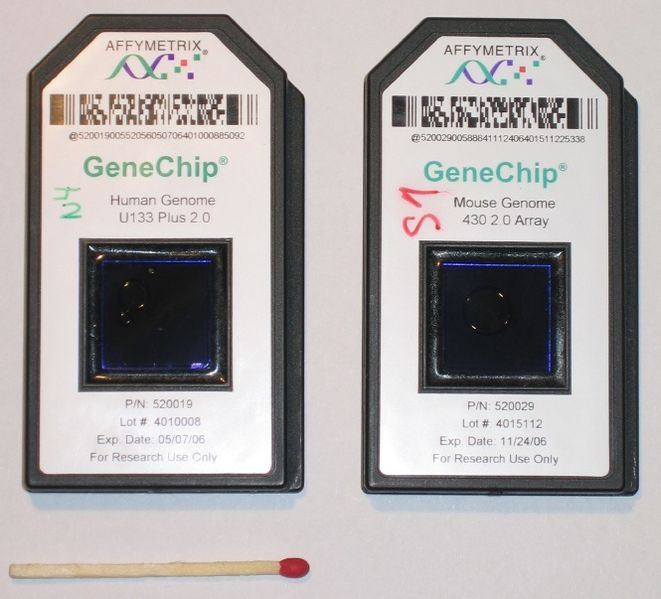
\includegraphics[width=0.9\textwidth]{Affymetrix-microarray}
      \end{figure}
    \end{column}
    \begin{column}{0.5\textwidth}
      \begin{figure}
        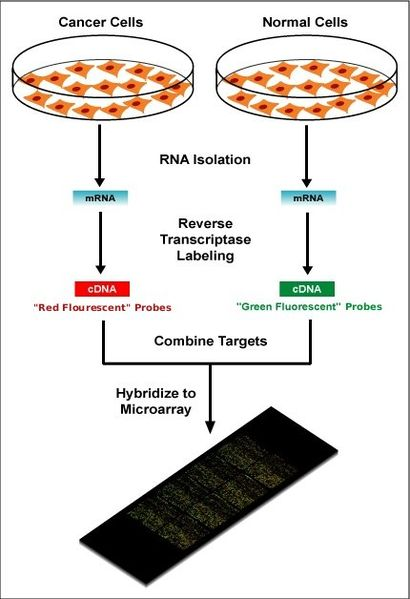
\includegraphics[width=0.9\textwidth]{Microarray-schema}
      \end{figure}
    \end{column}
  \end{columns}
  \source{en.wikipedia.org}
  \note{http://en.wikipedia.org/wiki/DNA_microarray}
\end{frame}

\begin{frame}[plain]
  \frametitle{Van't Veer breast-cancer data}
\begin{figure}
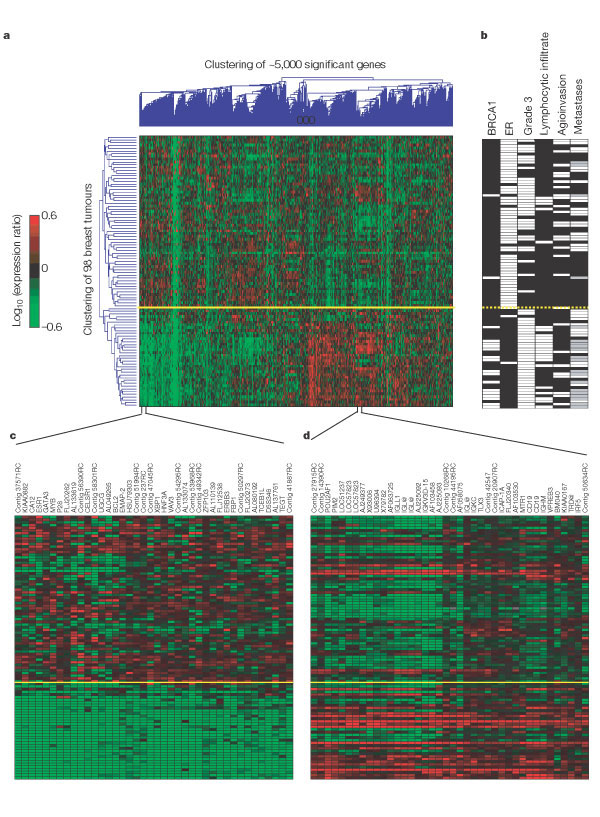
\includegraphics[height=1\textheight]{vantveer-summary}
\end{figure}
\mycite{Laura J. van 't Veer et.al. Nature, (2002)}
\note{a, Two-dimensional presentation of transcript ratios for 98 breast tumours. There were 4,968 significant genes across the group. Each row represents a tumour and each column a single gene. As shown in the colour bar, red indicates upregulation, green downregulation, black no change, and grey no data available. The yellow line marks the subdivision into two dominant tumour clusters. b, Selected clinical data for the 98 patients in a: BRCA1 germline mutation carrier (or sporadic patient), ER expression, tumour grade 3 (versus grade 1 and 2), lymphocytic infiltrate, angioinvasion, and metastasis status. White indicates positive, black negative and grey denotes tumours derived from BRCA1 germline carriers who were excluded from the metastasis evaluation. The cluster below the yellow line consists of 36 tumours, of which 34 are ER negative (total 39 ER-negative) and 16 are carriers of the BRCA1 mutation (total 18). c, Enlarged portion from a containing a group of genes that co-regulate with the ER- gene (ESR1). Each gene is labelled by its gene name or accession number from GenBank. Contig ESTs ending with RC are reverse-complementary of the named contig EST. d, Enlarged portion from a containing a group of co-regulated genes that are the molecular reflection of extensive lymphocytic infiltrate, and comprise a set of genes expressed in T and B cells. (Gene annotation as in c.)}
\note{http://www.nature.com/nature/journal/v415/n6871/full/415530a.html}
\end{frame}

\begin{frame}[plain]
  \frametitle{Yeast Protein Interaction Network}
\begin{figure}
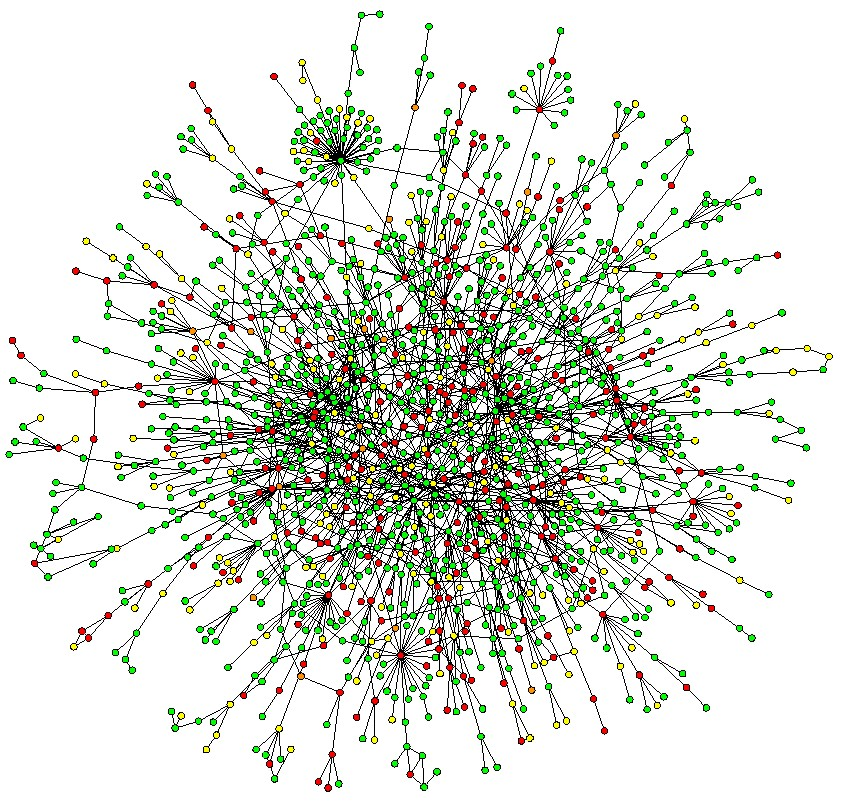
\includegraphics[width=0.8\textwidth]{yeastProteinInteractionNetwork}
\end{figure}
\note{http://www.bordalierinstitute.com/images/yeastProteinInteractionNetwork.jpg}
\source{http://osf1.gmu.edu/~rcouch/chem665.htm}
\end{frame}


\section{Formulation} 

\begin{frame}
\begin{figure}
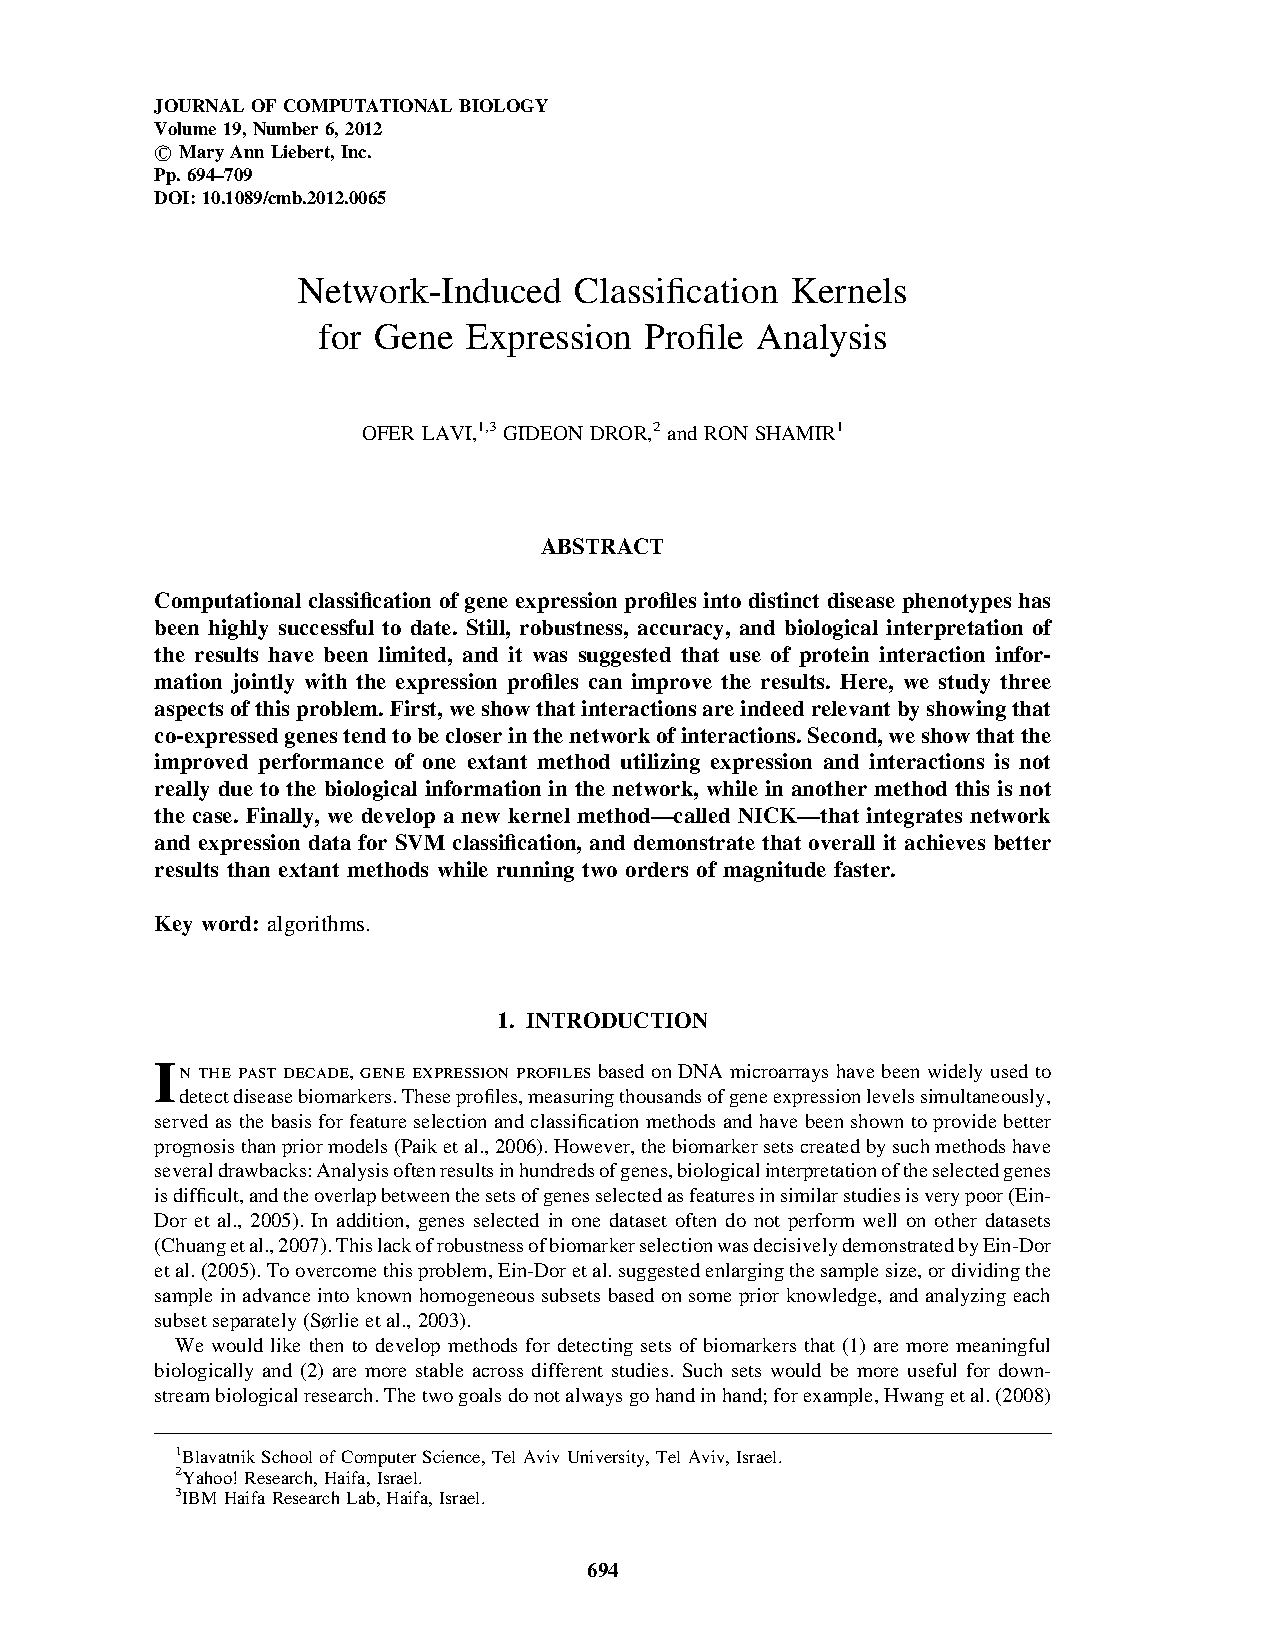
\includegraphics[height=1\textheight]{NICK-page1}
\end{figure}
\end{frame}


\begin{frame}
  \frametitle{NICK}
  \begin{columns}
    \begin{column}{0.5\textwidth}
      
      \begin{block}{\tiny{1. SVM modified objective function}}
        \tiny
        \begin{center}
          $\min_{\mathbf{w}, w_0}\left\{\frac{1}{2}\|\mathbf{w}\|^2 + \frac{1}{2}\beta\sum_{(j,k)\in E}(w_j-w_k)^2\right\}$
        \end{center}
        s.t.:
        \begin{center}
          $\forall i \in \{1,\cdots,n\} : (\mathbf{w}\mathbf{x}_i+w_0)y_i\geq 1$
        \end{center}
      \end{block}
      
      \begin{block}{\tiny{3. Dual to Primal}}
        \tiny
        \begin{center}
          $\mathbf{w} = (\mathbf{I} + \beta \mathbf{B})^{-1} \sum_{i = 1}^n \alpha_i y_i \mathbf{x}_i$
        \end{center}
      \end{block}
    \end{column}
    
    \begin{column}{0.5\textwidth}
      \begin{block}{\tiny{2. Dual problem}}
        \tiny
        \begin{center}
          \begin{align*}
            &\max_\alpha\left\{\sum_{i=1}^n\alpha_i-\frac{1}{2}\sum_{i=1}^n\sum_{j=1}^n\alpha_i\alpha_j y_i y_j (\mathbf{x}_i^T\mathbf{L})(\mathbf{L}^T\mathbf{x}_j)\right\}\\
            &\mathbf{L}\mathbf{L}^T=(\mathbf{I}+\beta \mathbf{B})^{-1}\\
            \text{s.t.: }&\\
            &\forall i \in \{1,\cdots,n\}: \sum_{i=1}^n\alpha_iy_i=0\\
            &\forall i \in \{1,\cdots,n\}: \alpha_i \geq 0
          \end{align*}
        \end{center}
      \end{block}
    \end{column}
  \end{columns}
  \mycite{Ofer Lavi, et.al., Journal of Computational Biology, (2012)}
\end{frame}

\begin{frame}
  \frametitle{NICK Performance Summary}
  \begin{figure}
    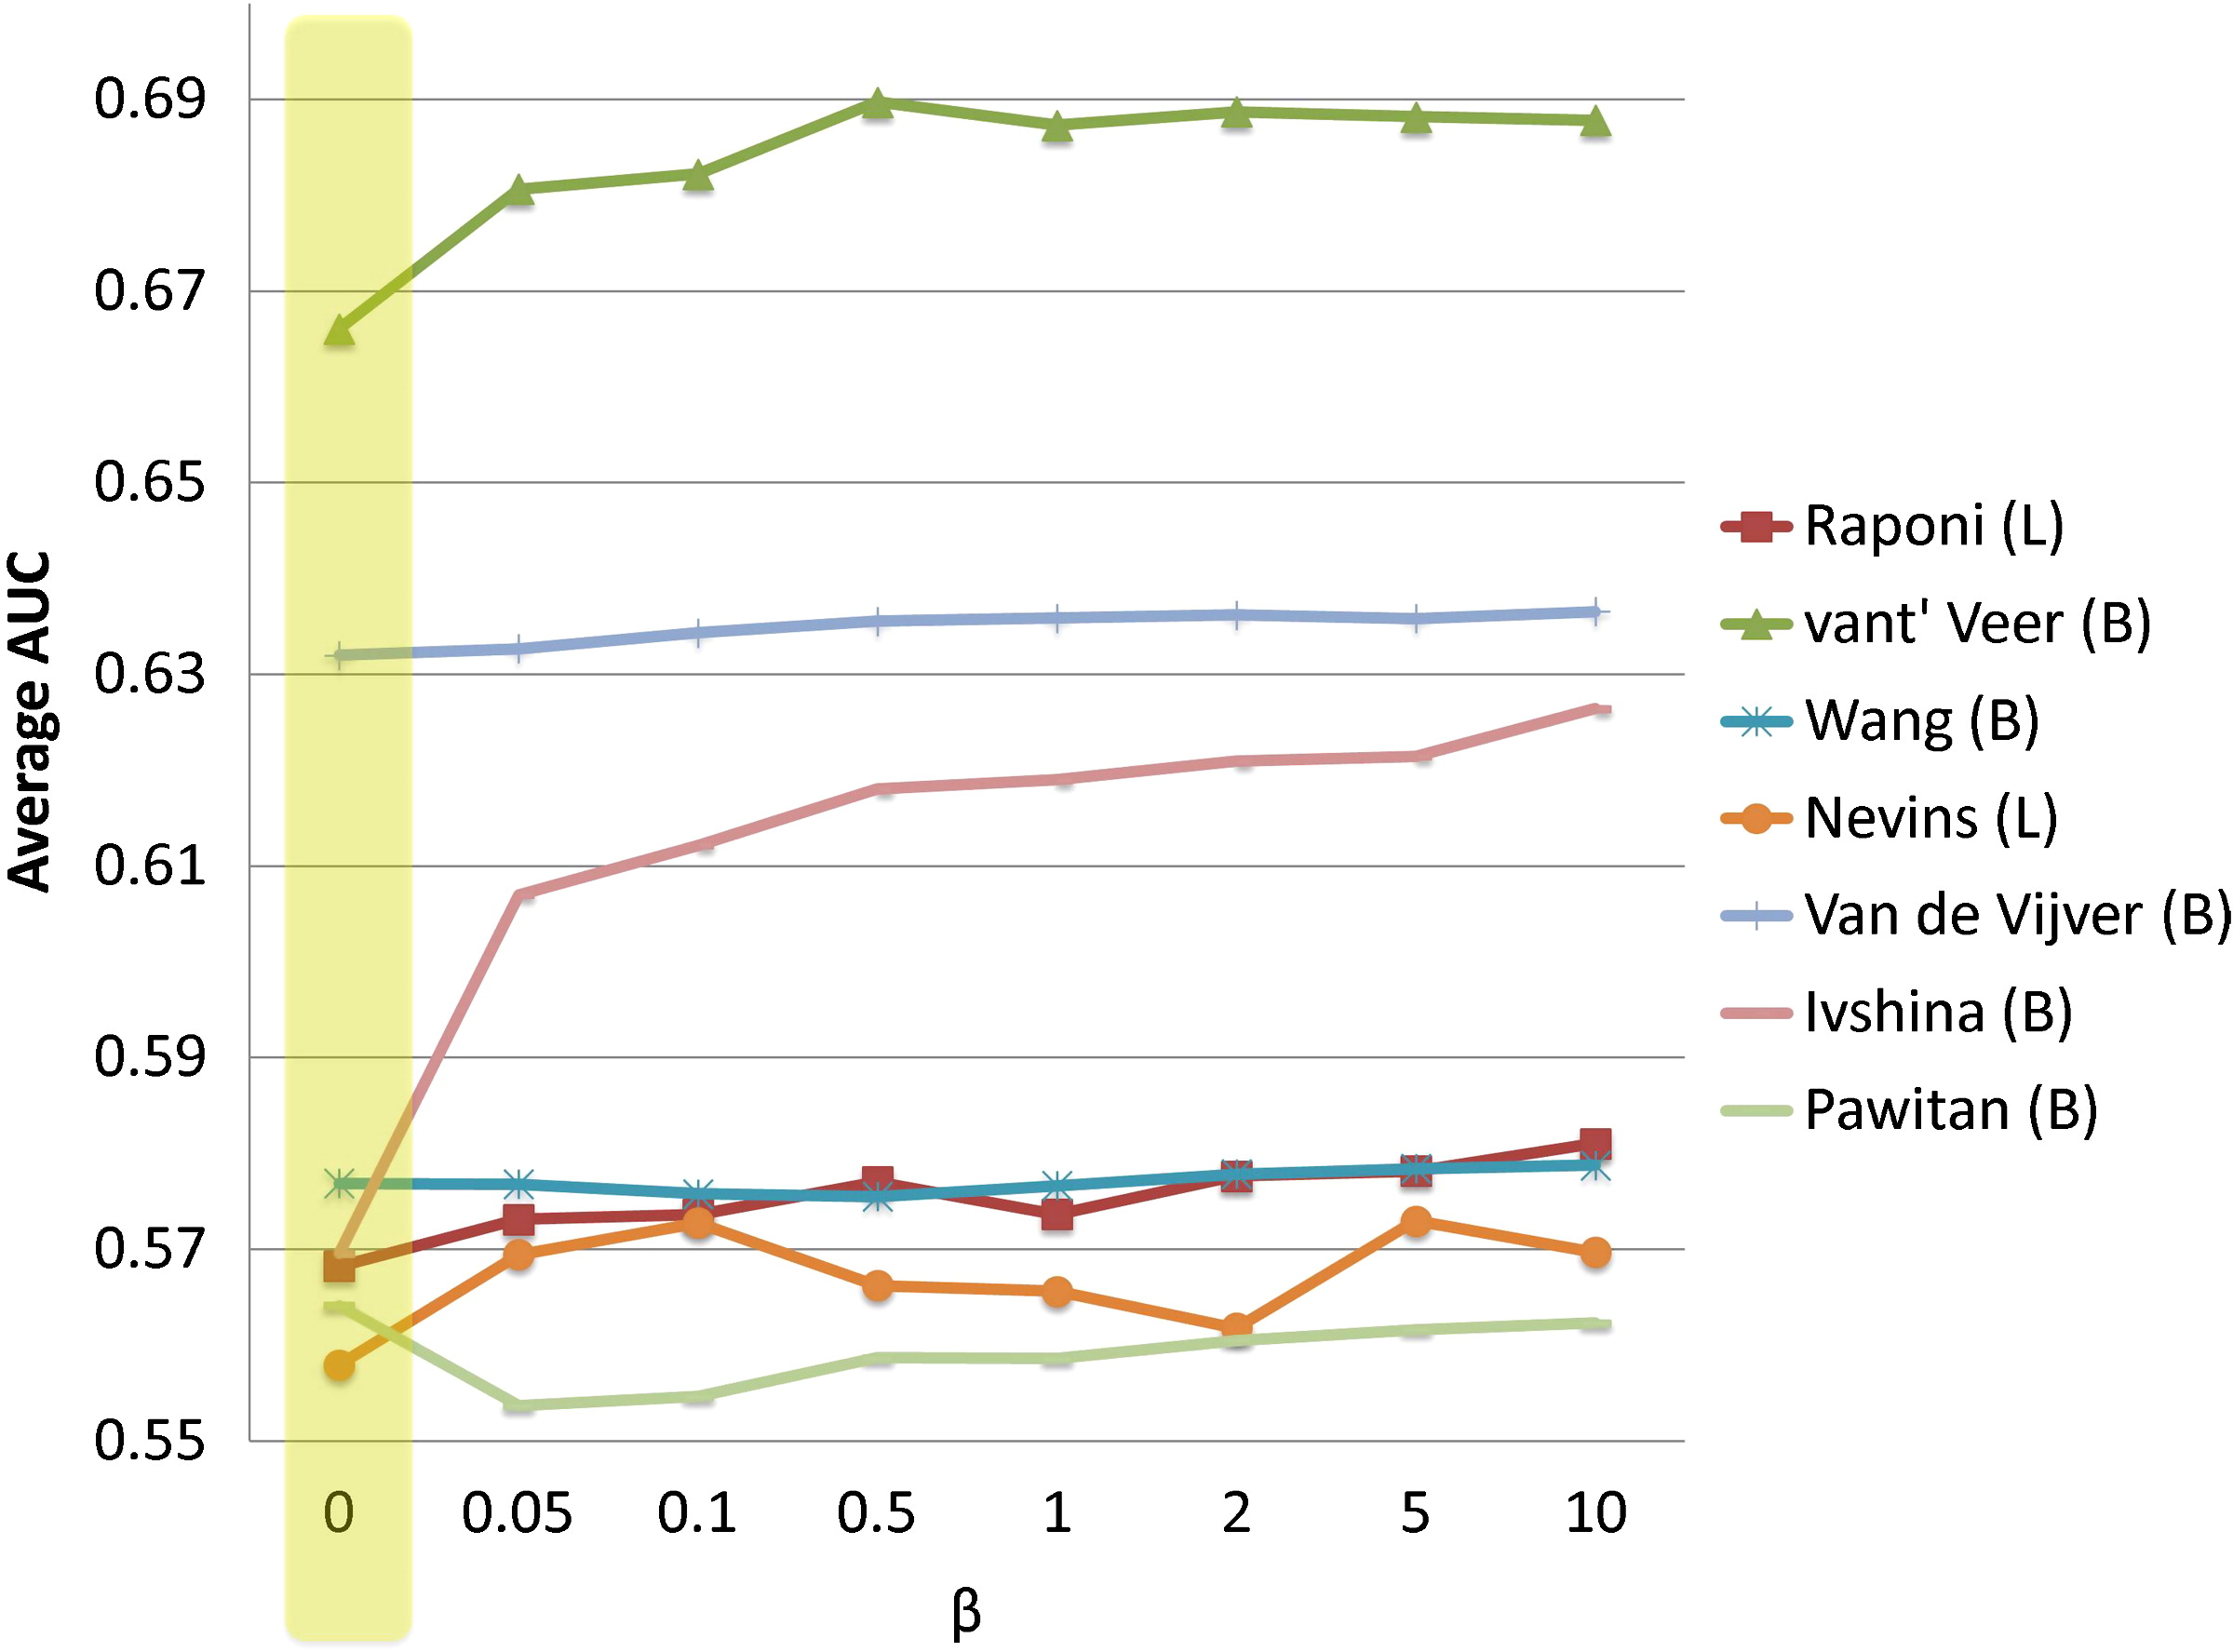
\includegraphics[width=0.8\textwidth]{NICK-perfs}
  \end{figure}
  \mycite{Ofer Lavi, et.al., Journal of Computational Biology, (2012)}
  \note{http://online.liebertpub.com/doi/full/10.1089/cmb.2012.0065}
\end{frame}


\section{Results}
\begin{frame}
\frametitle{Synthesize data}
\begin{enumerate}
\item A random graph
\item Signal nodes: \[ f(n) = \left\{ 
  \begin{array}{l l}
    N(-\mu, 1) & \quad \text{if $n$ is in class $1$}\\
    N(\mu, 1) & \quad \text{if $n$ is in class $2$}
  \end{array} \right.\]
\item Random nodes: \[f(n) = N(0, 1) \]
\item Pathway: 2, 3, or 4 connected signal nodes.
\end{enumerate}
\end{frame}

\begin{frame}[plain]
  \frametitle{Synthesized data}
\only<1-2>{
  \begin{figure}
    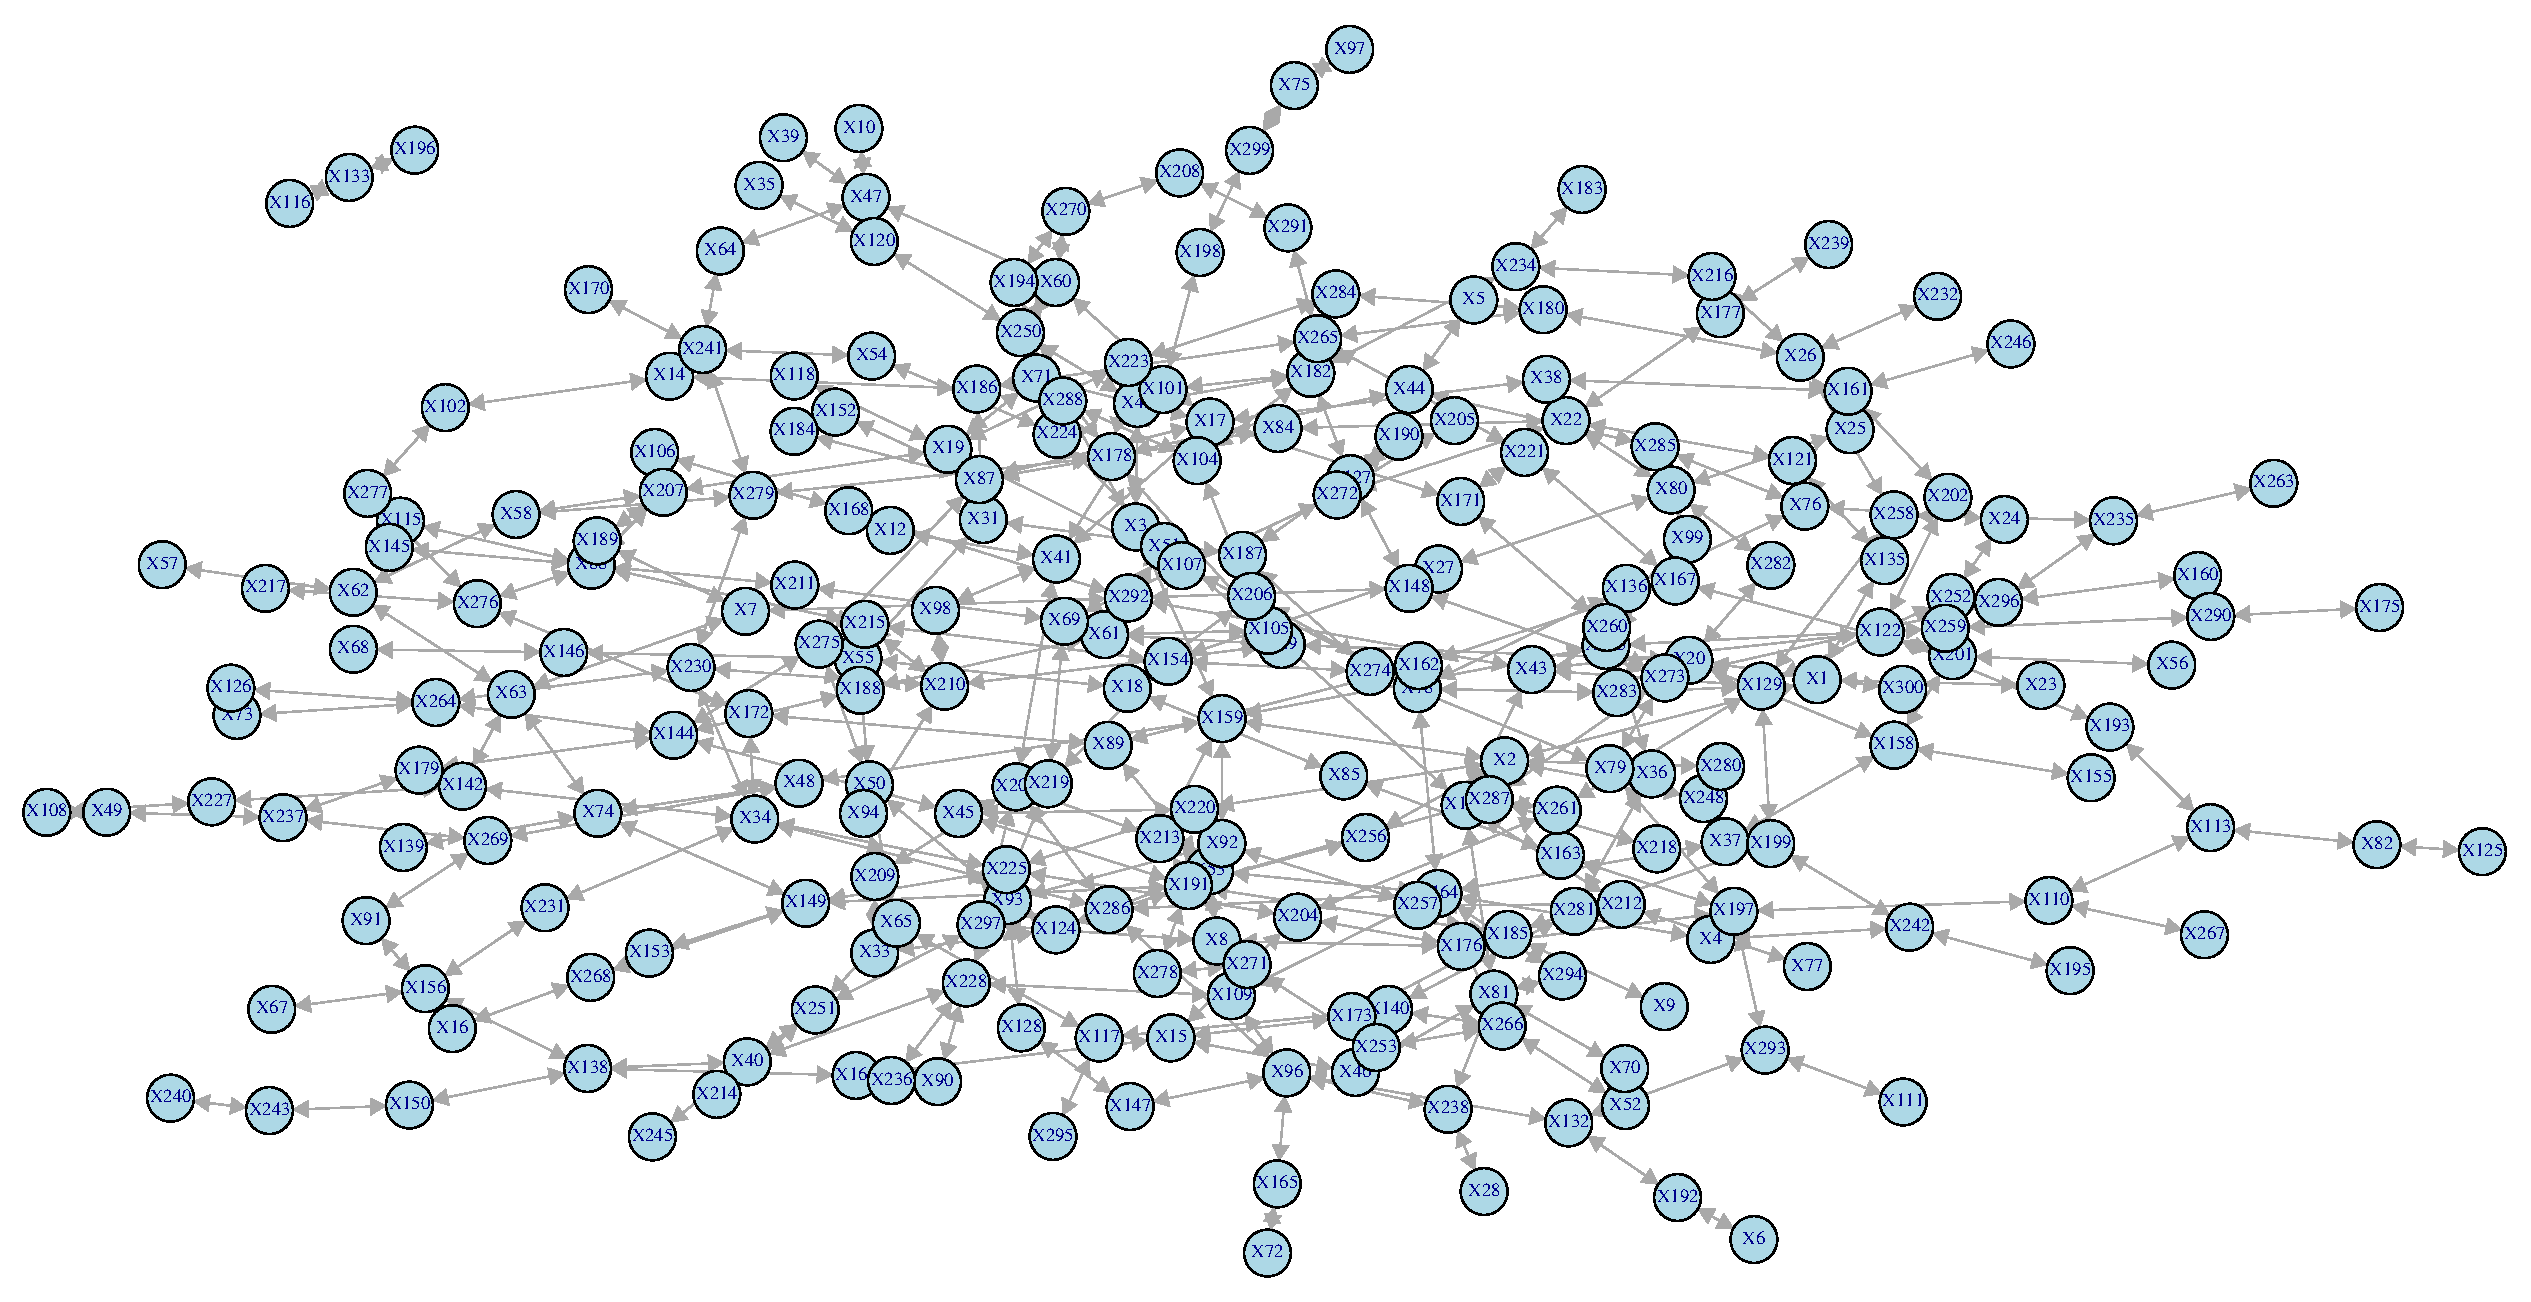
\includegraphics[width=0.8\textwidth]{synthesized}
  \end{figure}
}
\only<2-3>{
  \begin{textblock*}{\paperwidth}(0.4\textwidth,0.8\textheight)
    \raggedright
  \begin{figure}
    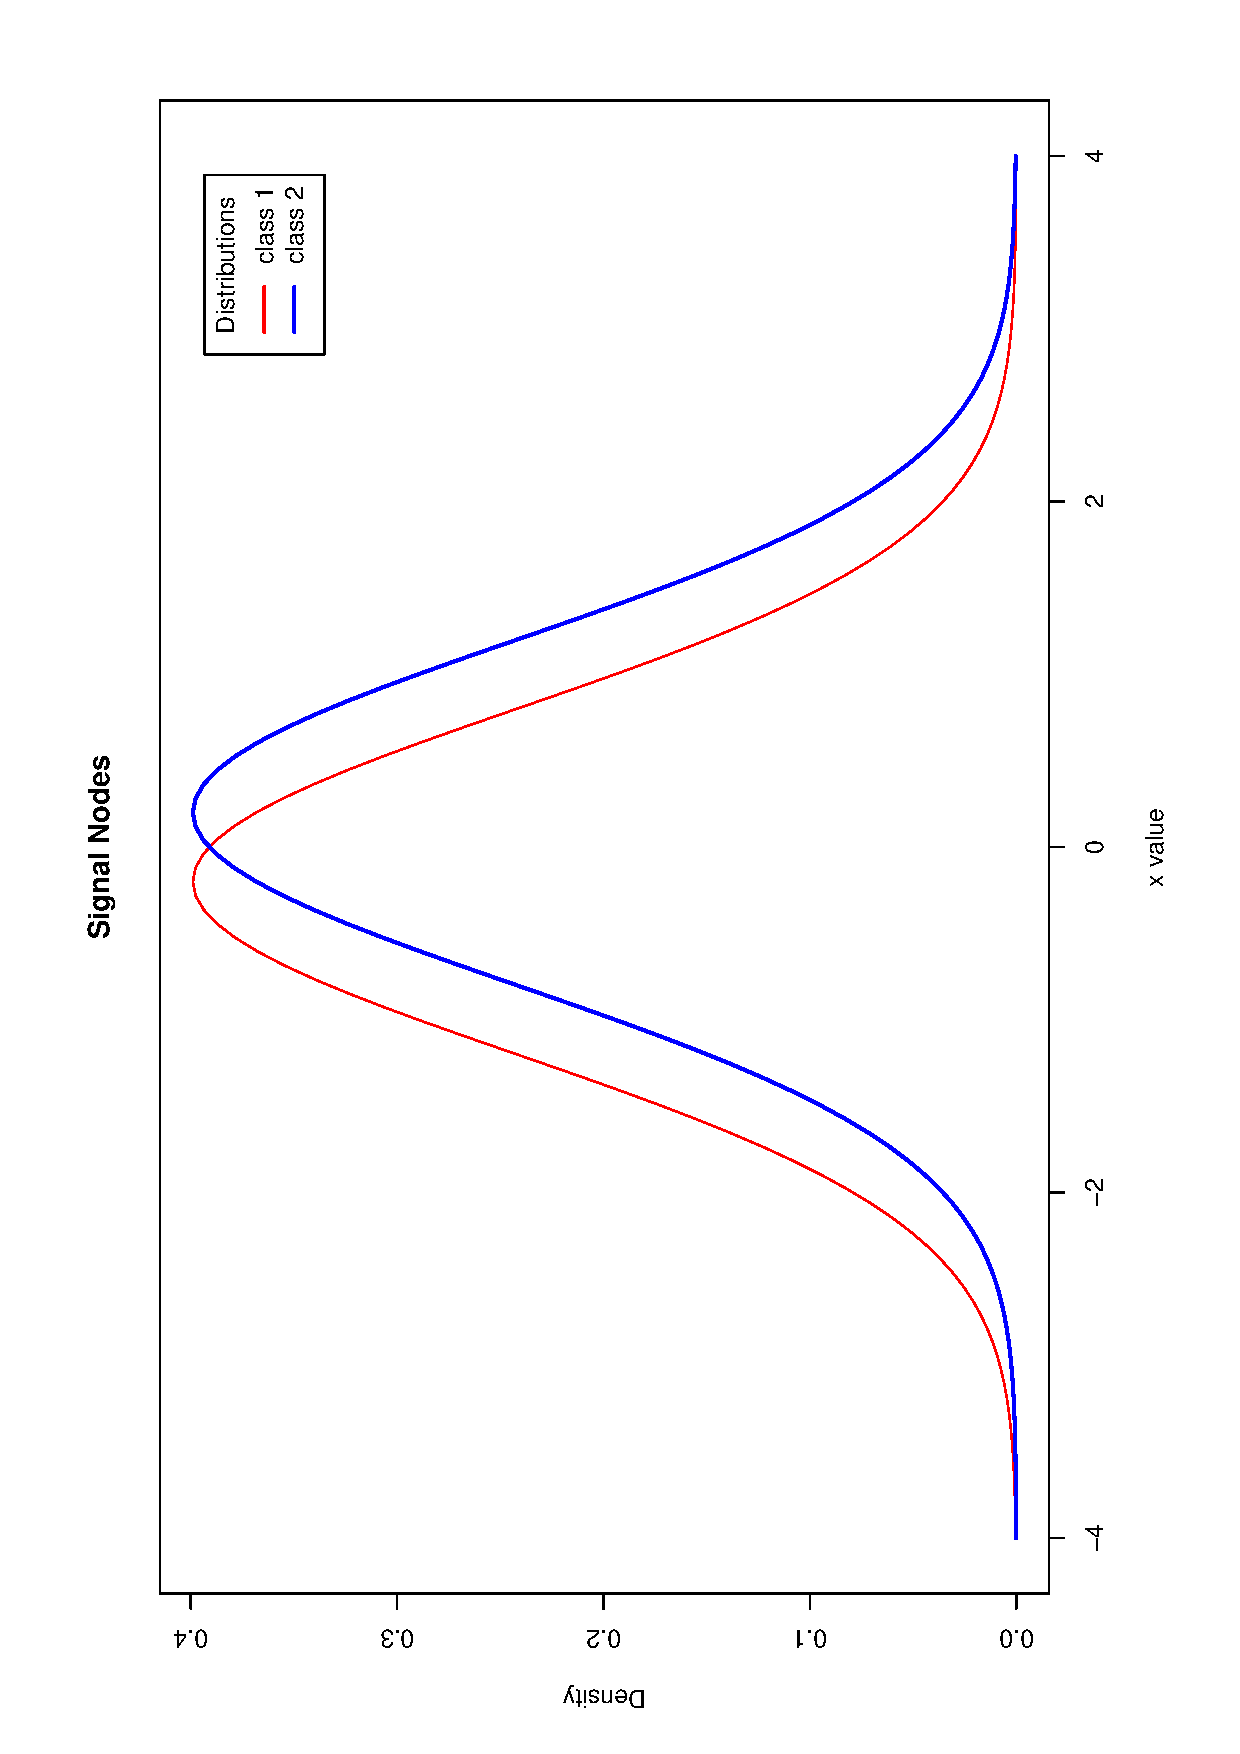
\includegraphics[angle=270,width=0.2\textwidth]{signal-nodes}
  \end{figure}
  \end{textblock*}
  \begin{textblock*}{\paperwidth}(-0.4\textwidth,0.8\textheight)
    \raggedright
  \begin{figure}
    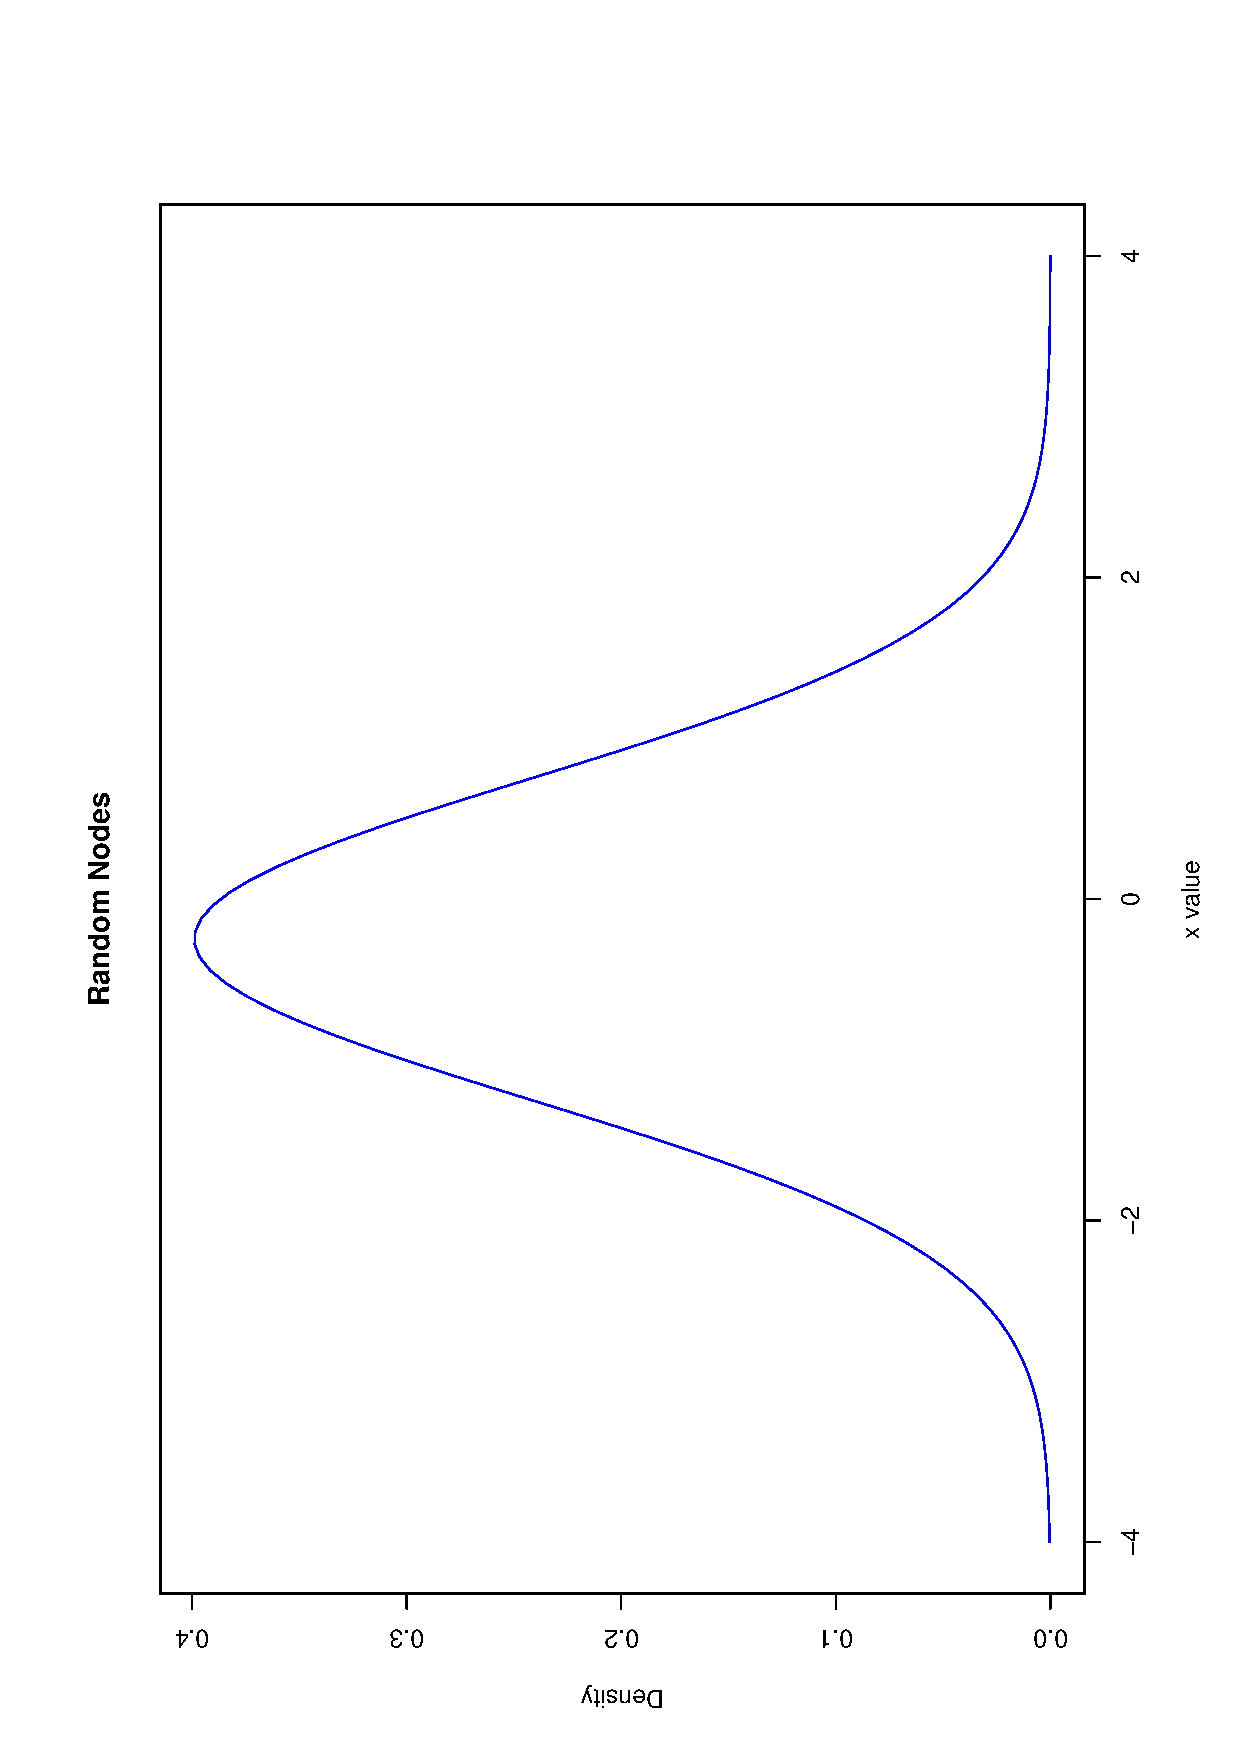
\includegraphics[angle=270,width=0.2\textwidth]{random-nodes}
  \end{figure}
  \end{textblock*}
}
\only<3>{
  \begin{figure}
    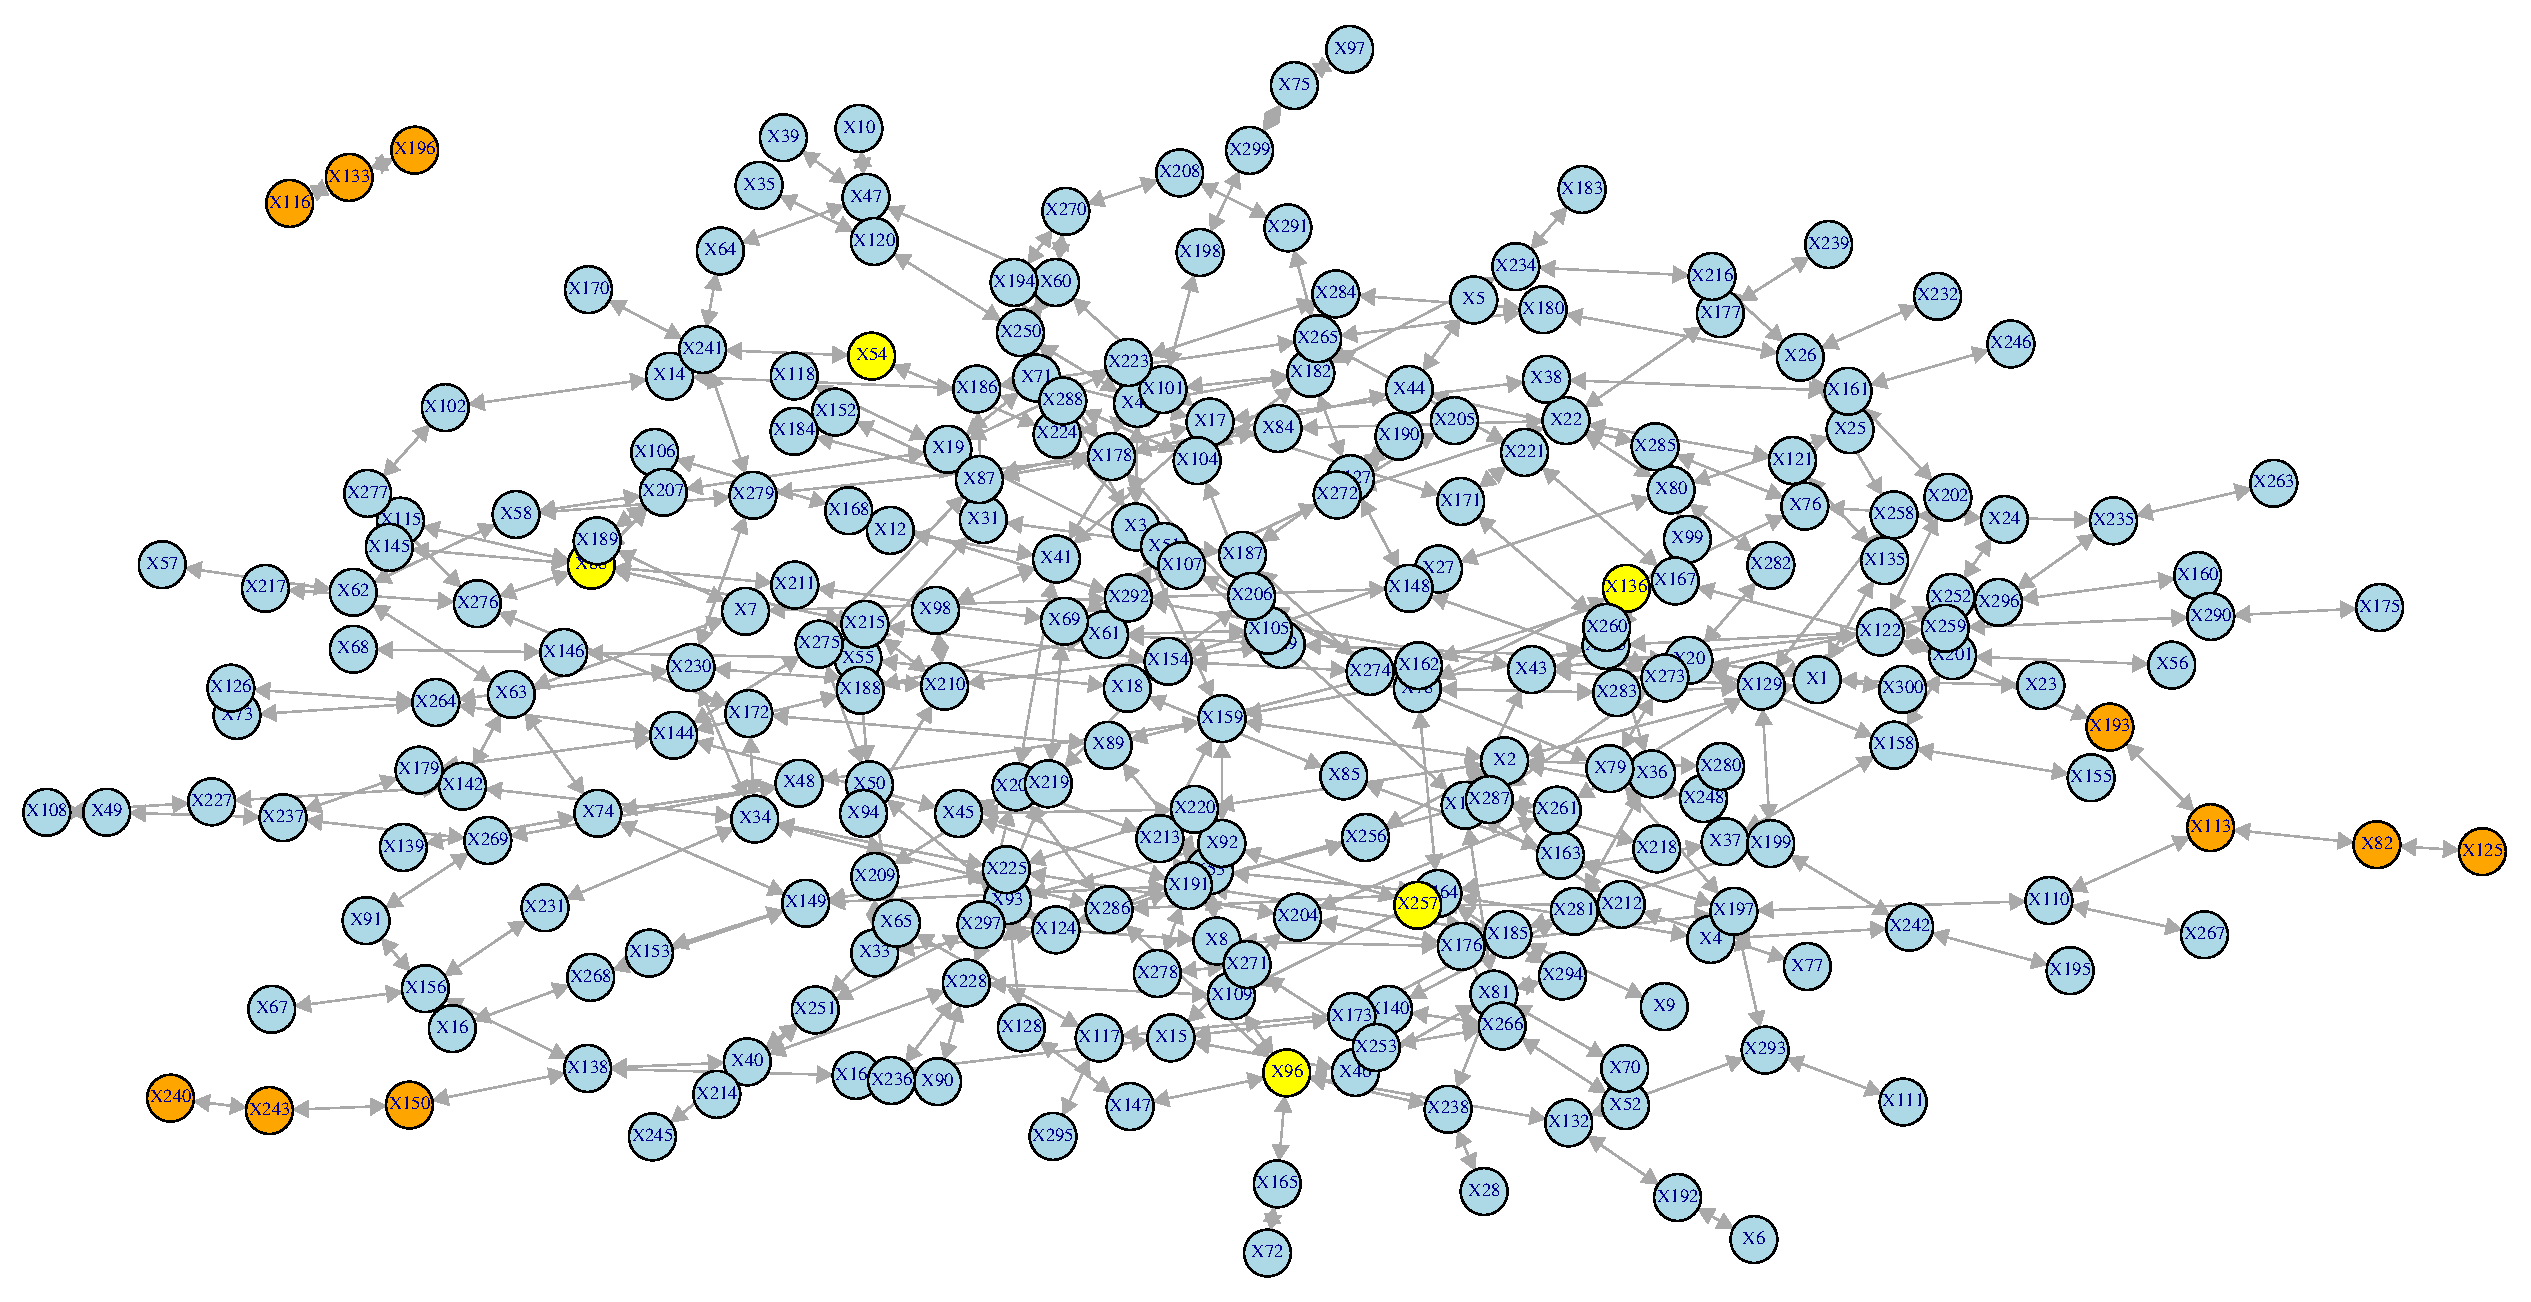
\includegraphics[width=0.8\textwidth]{synthesized-easy}
  \end{figure}
}
\end{frame}

\begin{frame}[plain]
  \frametitle{Synthesized data easy scenario}
  \begin{figure}
    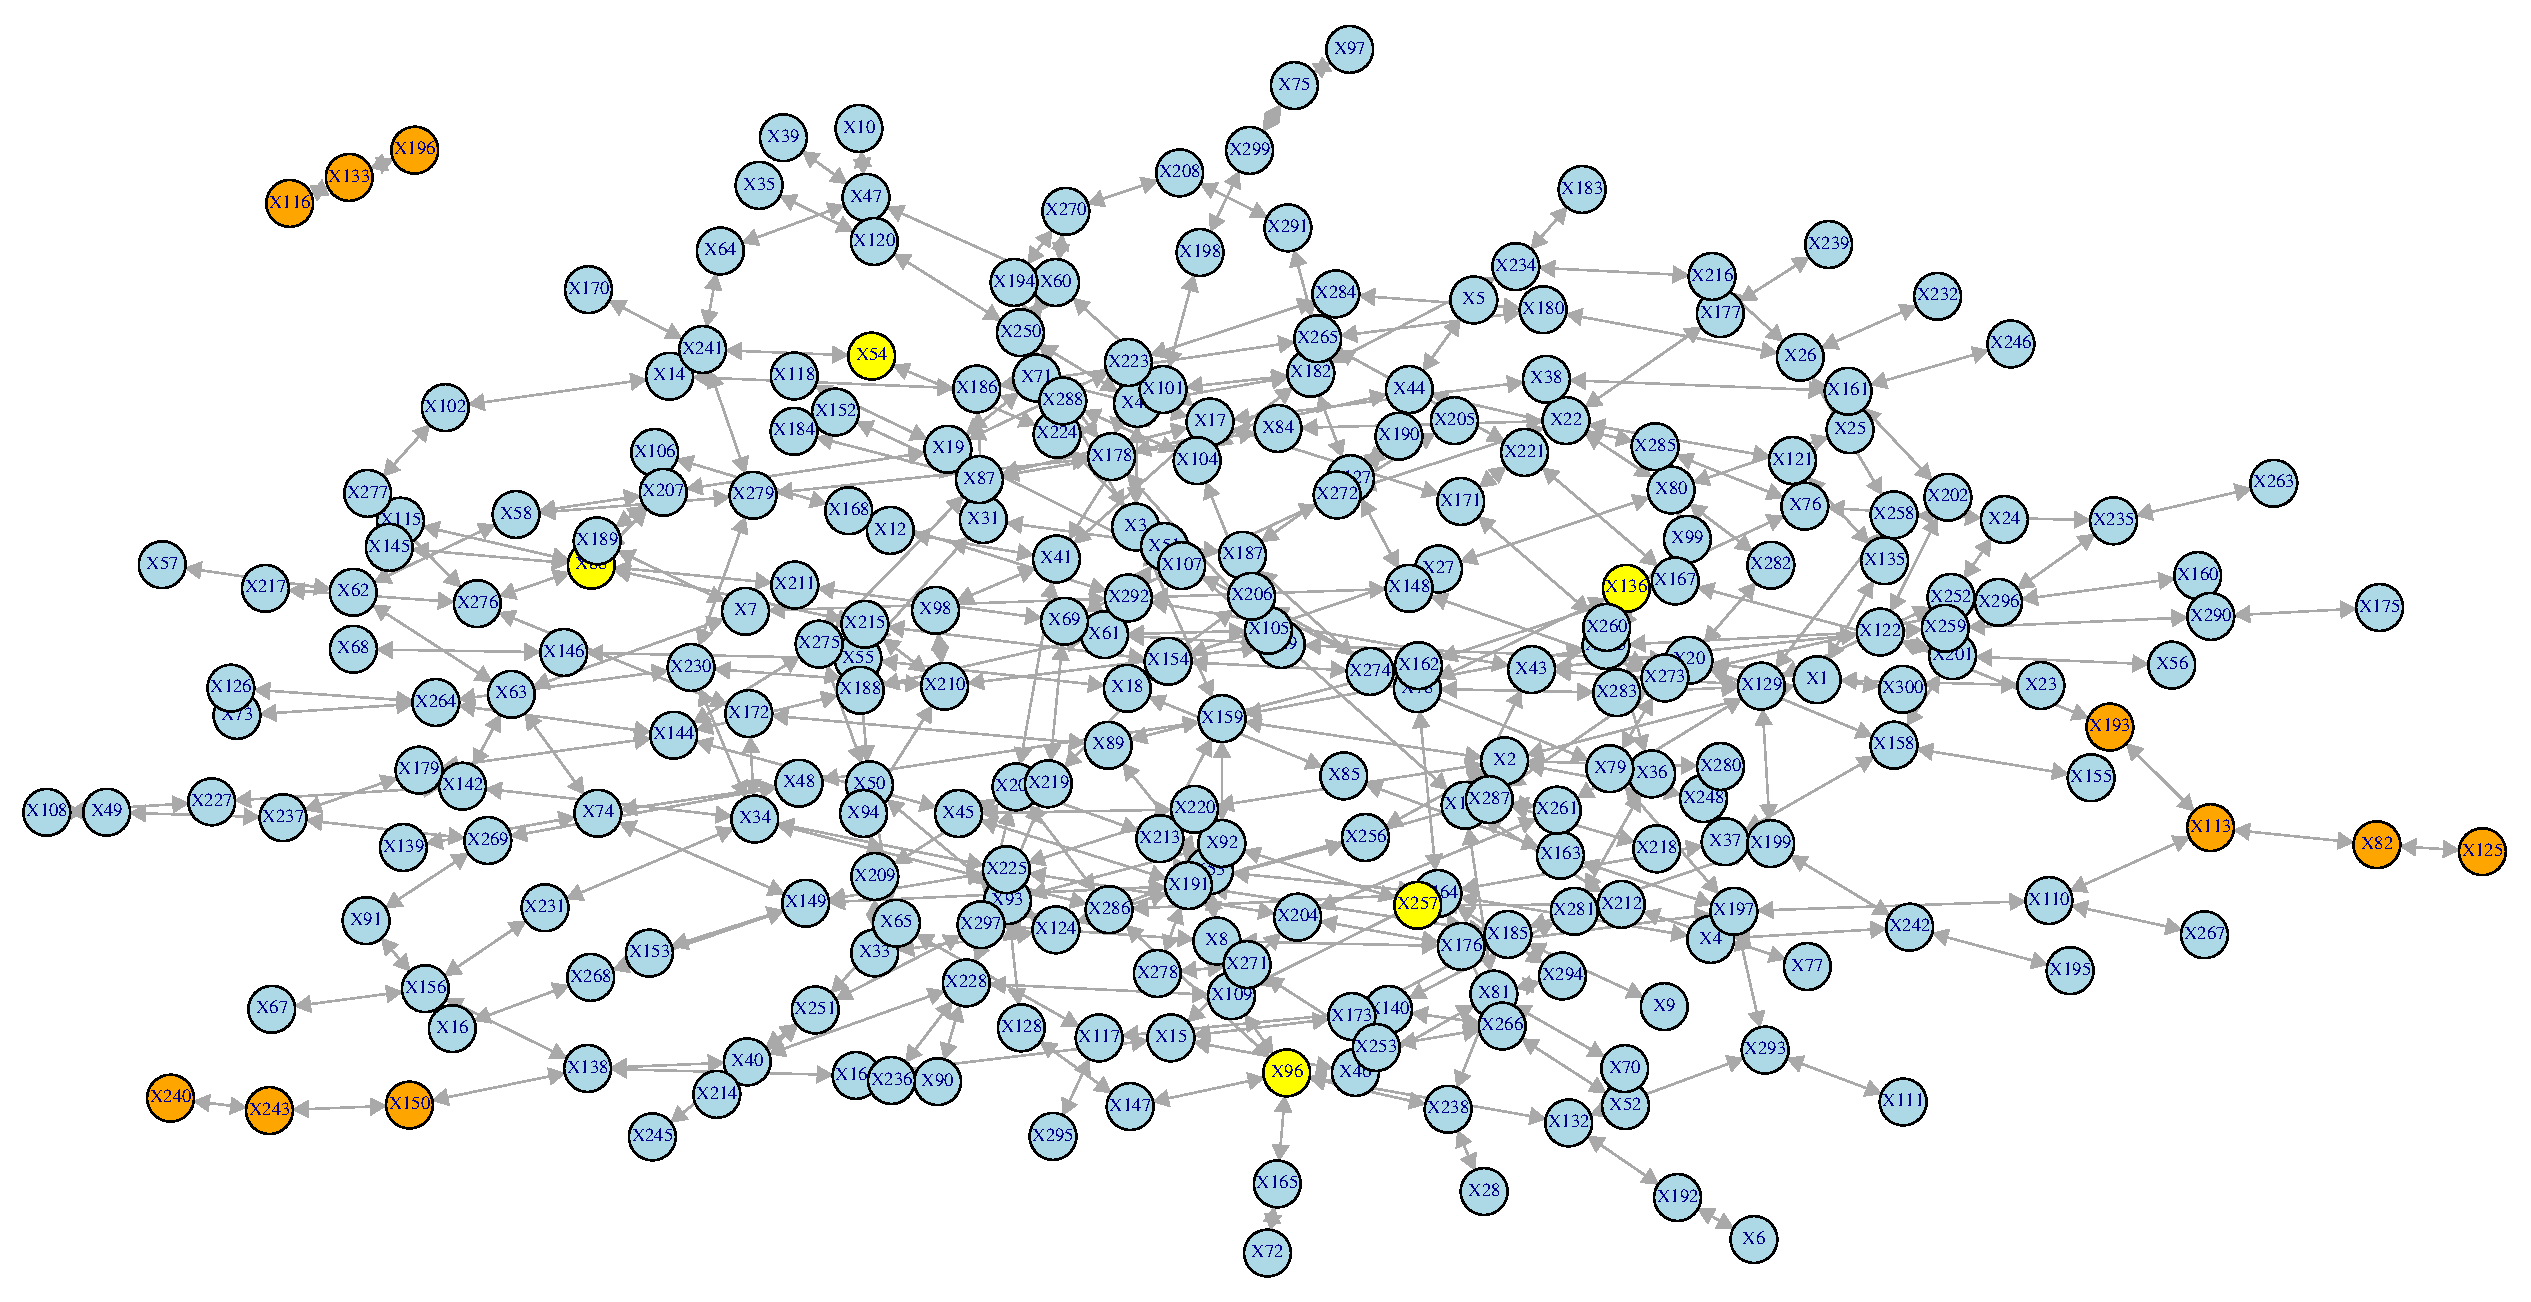
\includegraphics[width=0.8\textwidth]{synthesized-easy}
  \end{figure}
  \begin{textblock*}{\paperwidth}(0.01\textwidth,0.15\textheight)
    \raggedright 
    \tiny
    \begin{tabular}{| c c |}
      \hline
AUC: & 60.6 \\ \hline \hline
\boz X196   &  \boz X196  \\ \hline
X53   &  X53  \\ \hline
X233   &  X233  \\ \hline
X39   &  X39  \\ \hline
\ghool X88   &  \ghool X88  \\ \hline
\boz X196   &  \boz X133  \\ \hline
\boz X116   &  \boz X116  \\ \hline
X127   &  X127  \\ \hline
X197   &  X197  \\ \hline
X127   &  X148  \\ \hline
X148   &  X148  \\ \hline
\boz X150   &  \boz X150  \\ \hline
X148   &  X273  \\ \hline
\boz X116   &  \boz X133  \\ \hline
X160   &  X160  \\ \hline
\ghool X96   &  \ghool X96  \\ \hline
X95   &  X95  \\ \hline
X273   &  X273  \\ \hline
\ghool X88   &  X115  \\ \hline
X40   &  X40  \\ \hline
X53   &  X8  \\ \hline
X53   &  X164  \\ \hline
X195   &  X195  \\ \hline
X56   &  X56  \\ \hline
\boz X113   &  \boz X113  \\ \hline
X179   &  X179  \\ \hline
\ghool X96   &  X147  \\ \hline
\boz X240   &  \boz X240  \\ \hline
X197   &  X110  \\ \hline
X197   &  X293  \\ \hline
    \end{tabular}
    \hspace{.5em}
  \end{textblock*}
  \begin{textblock*}{\paperwidth}(1\textwidth,0.15\textheight)
    \raggedright 
    \tiny
    \begin{tabular}{| c c |}
      \hline
AUC: & 62.4 \\ \hline \hline
\boz X196   &  \boz X196  \\ \hline
X233   &  X233  \\ \hline
\boz X196   &  \boz X133  \\ \hline
\boz X133   &  \boz X133  \\ \hline
\boz X133   &  \boz X116  \\ \hline
\boz X116   &  \boz X116  \\ \hline
X95   &  X95  \\ \hline
\boz X240   &  \boz X240  \\ \hline
X39   &  X39  \\ \hline
\boz X240   &  \boz X243  \\ \hline
X59   &  X59  \\ \hline
X106   &  X106  \\ \hline
\boz X243   &  \boz X243  \\ \hline
X106   &  X168  \\ \hline
X114   &  X114  \\ \hline
X168   &  X168  \\ \hline
\boz X243   &  \boz X150  \\ \hline
X56   &  X56  \\ \hline
X39   &  X47  \\ \hline
X298   &  X298  \\ \hline
\boz X150   &  \boz X150  \\ \hline
X247   &  X247  \\ \hline
\boz X125   &  \boz X125  \\ \hline
X83   &  X83  \\ \hline
\boz X125   &  \boz X82  \\ \hline
\boz X82   &  \boz X82  \\ \hline
X160   &  X160  \\ \hline
X195   &  X195  \\ \hline
\boz X196   &  \boz X116  \\ \hline
\boz X82   &  \boz X113  \\ \hline
    \end{tabular}
    \hspace{.5em}
  \end{textblock*}
  \begin{textblock*}{\paperwidth}(0.4\textwidth,1.1\textheight)
    \raggedright 
    \tiny
    \begin{tabular}{| c c |}
      \hline
      wc p-value (paired): & 5.669e-09 \\ \hline
    \end{tabular}
    \hspace{.5em}
  \end{textblock*}
\end{frame}

\begin{frame}[plain]
  \frametitle{Synthesized data medium scenario}
  \begin{figure}
    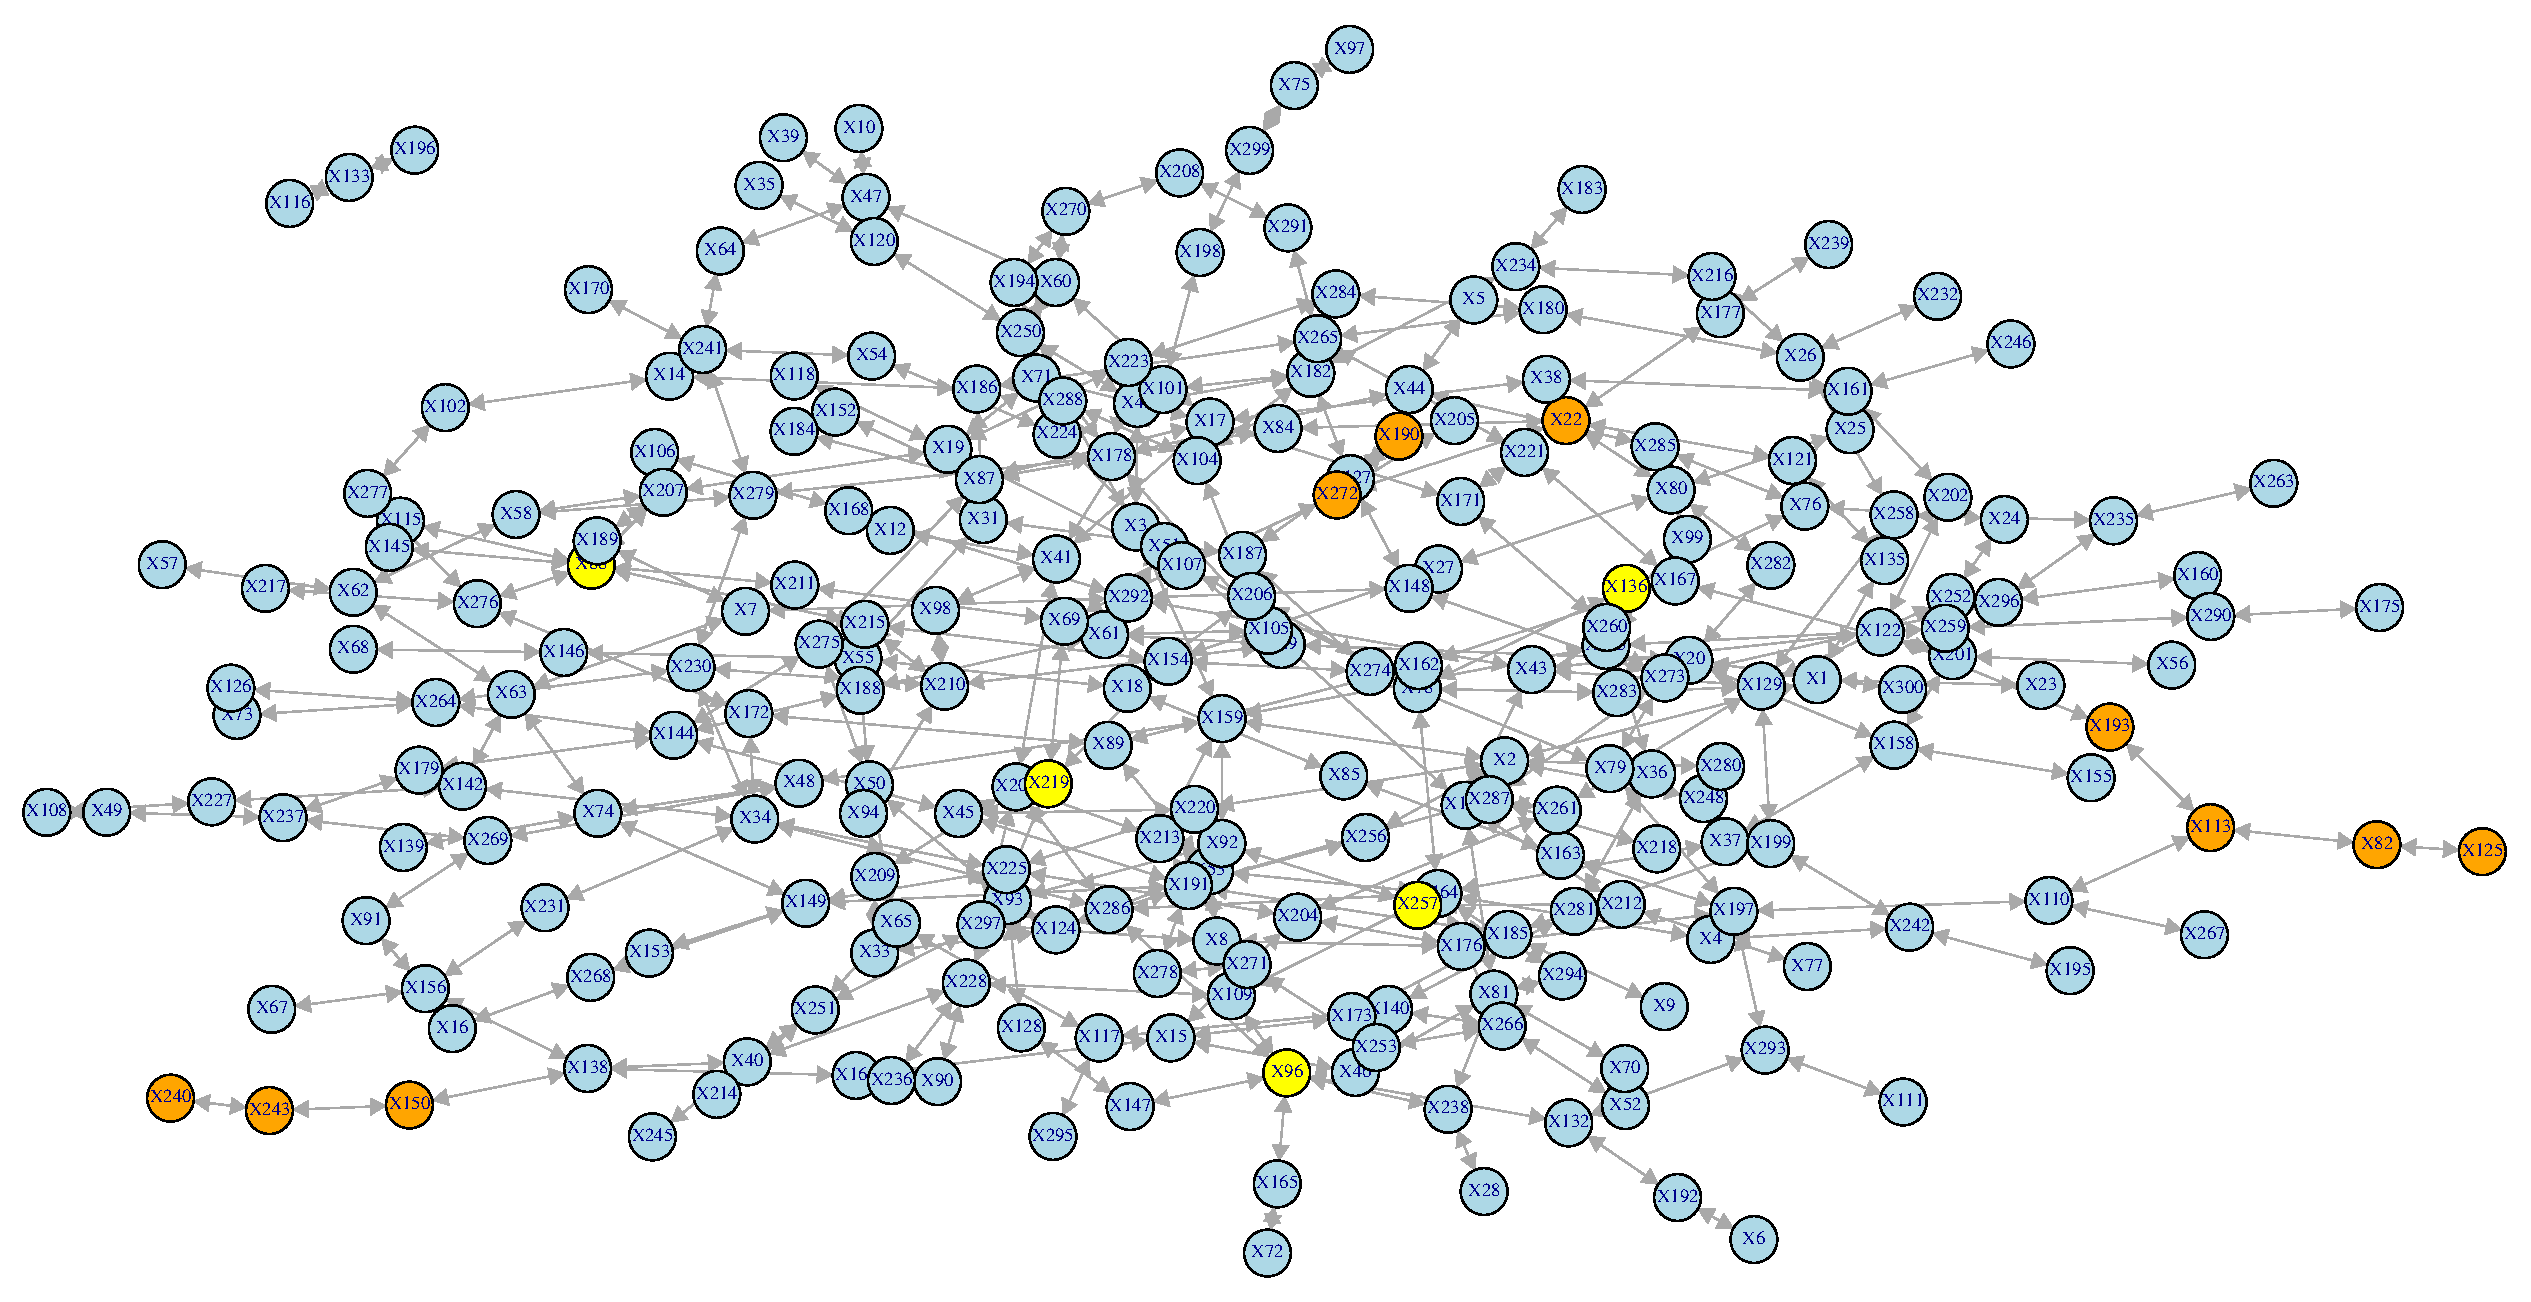
\includegraphics[width=0.8\textwidth]{synthesized-medium}
  \end{figure}
  \begin{textblock*}{\paperwidth}(0.01\textwidth,0.15\textheight)
    \raggedright 
    \tiny
    \begin{tabular}{| c c |}
      \hline
AUC: & 60.1 \\ \hline \hline
\boz X190   &  \boz X190  \\ \hline
X104   &  X104  \\ \hline
X233   &  X233  \\ \hline
\boz X190   &  \boz X272  \\ \hline
X277   &  X277  \\ \hline
\ghool X88   &  \ghool X88  \\ \hline
\boz X190   &  X127  \\ \hline
X165   &  X165  \\ \hline
\boz X272   &  \boz X272  \\ \hline
\boz X272   &  \boz X22  \\ \hline
X106   &  X106  \\ \hline
X165   &  \ghool X96  \\ \hline
\boz X150   &  \boz X150  \\ \hline
X250   &  X250  \\ \hline
\ghool X88   &  X215  \\ \hline
\boz X22   &  \boz X22  \\ \hline
X51   &  X51  \\ \hline
X28   &  X28  \\ \hline
X73   &  X73  \\ \hline
X35   &  X35  \\ \hline
X162   &  X162  \\ \hline
\boz X113   &  \boz X113  \\ \hline
X112   &  X112  \\ \hline
X277   &  X102  \\ \hline
\ghool X96   &  \ghool X96  \\ \hline
X104   &  X206  \\ \hline
\ghool X88   &  X207  \\ \hline
X104   &  X182  \\ \hline
\ghool X96   &  X132  \\ \hline
X277   &  X276  \\ \hline
    \end{tabular}
    \hspace{.5em}
  \end{textblock*}
  \begin{textblock*}{\paperwidth}(1\textwidth,0.15\textheight)
    \raggedright 
    \tiny
    \begin{tabular}{| c c |}
      \hline
AUC: & 61.5 \\ \hline \hline
X233   &  X233  \\ \hline
\boz X190   &  \boz X190  \\ \hline
X112   &  X112  \\ \hline
\boz X240   &  \boz X240  \\ \hline
\boz X190   &  \boz X272  \\ \hline
\boz X240   &  \boz X243  \\ \hline
X86   &  X86  \\ \hline
\boz X243   &  \boz X243  \\ \hline
\boz X243   &  \boz X150  \\ \hline
\boz X190   &  X127  \\ \hline
\boz X150   &  \boz X150  \\ \hline
\boz X272   &  \boz X272  \\ \hline
X246   &  X246  \\ \hline
X298   &  X298  \\ \hline
X106   &  X106  \\ \hline
\boz X125   &  \boz X125  \\ \hline
X35   &  X35  \\ \hline
\boz X125   &  \boz X82  \\ \hline
X247   &  X247  \\ \hline
\boz X272   &  X69  \\ \hline
\boz X272   &  \boz X22  \\ \hline
\boz X82   &  \boz X82  \\ \hline
X100   &  X100  \\ \hline
\ghool X257   &  \ghool X257  \\ \hline
\boz X82   &  \boz X113  \\ \hline
X28   &  X28  \\ \hline
\boz X272   &  X205  \\ \hline
X131   &  X131  \\ \hline
\boz X113   &  \boz X113  \\ \hline
X246   &  X161  \\ \hline
    \end{tabular}
    \hspace{.5em}
  \end{textblock*}
  \begin{textblock*}{\paperwidth}(0.4\textwidth,1.1\textheight)
    \raggedright 
    \tiny
    \begin{tabular}{| c c |}
      \hline
      wc p-value (paired): & 1.383e-06 \\ \hline
    \end{tabular}
    \hspace{.5em}
  \end{textblock*}
\end{frame}

\begin{frame}[plain]
  \frametitle{Synthesized data hard scenario}
  \begin{figure}
    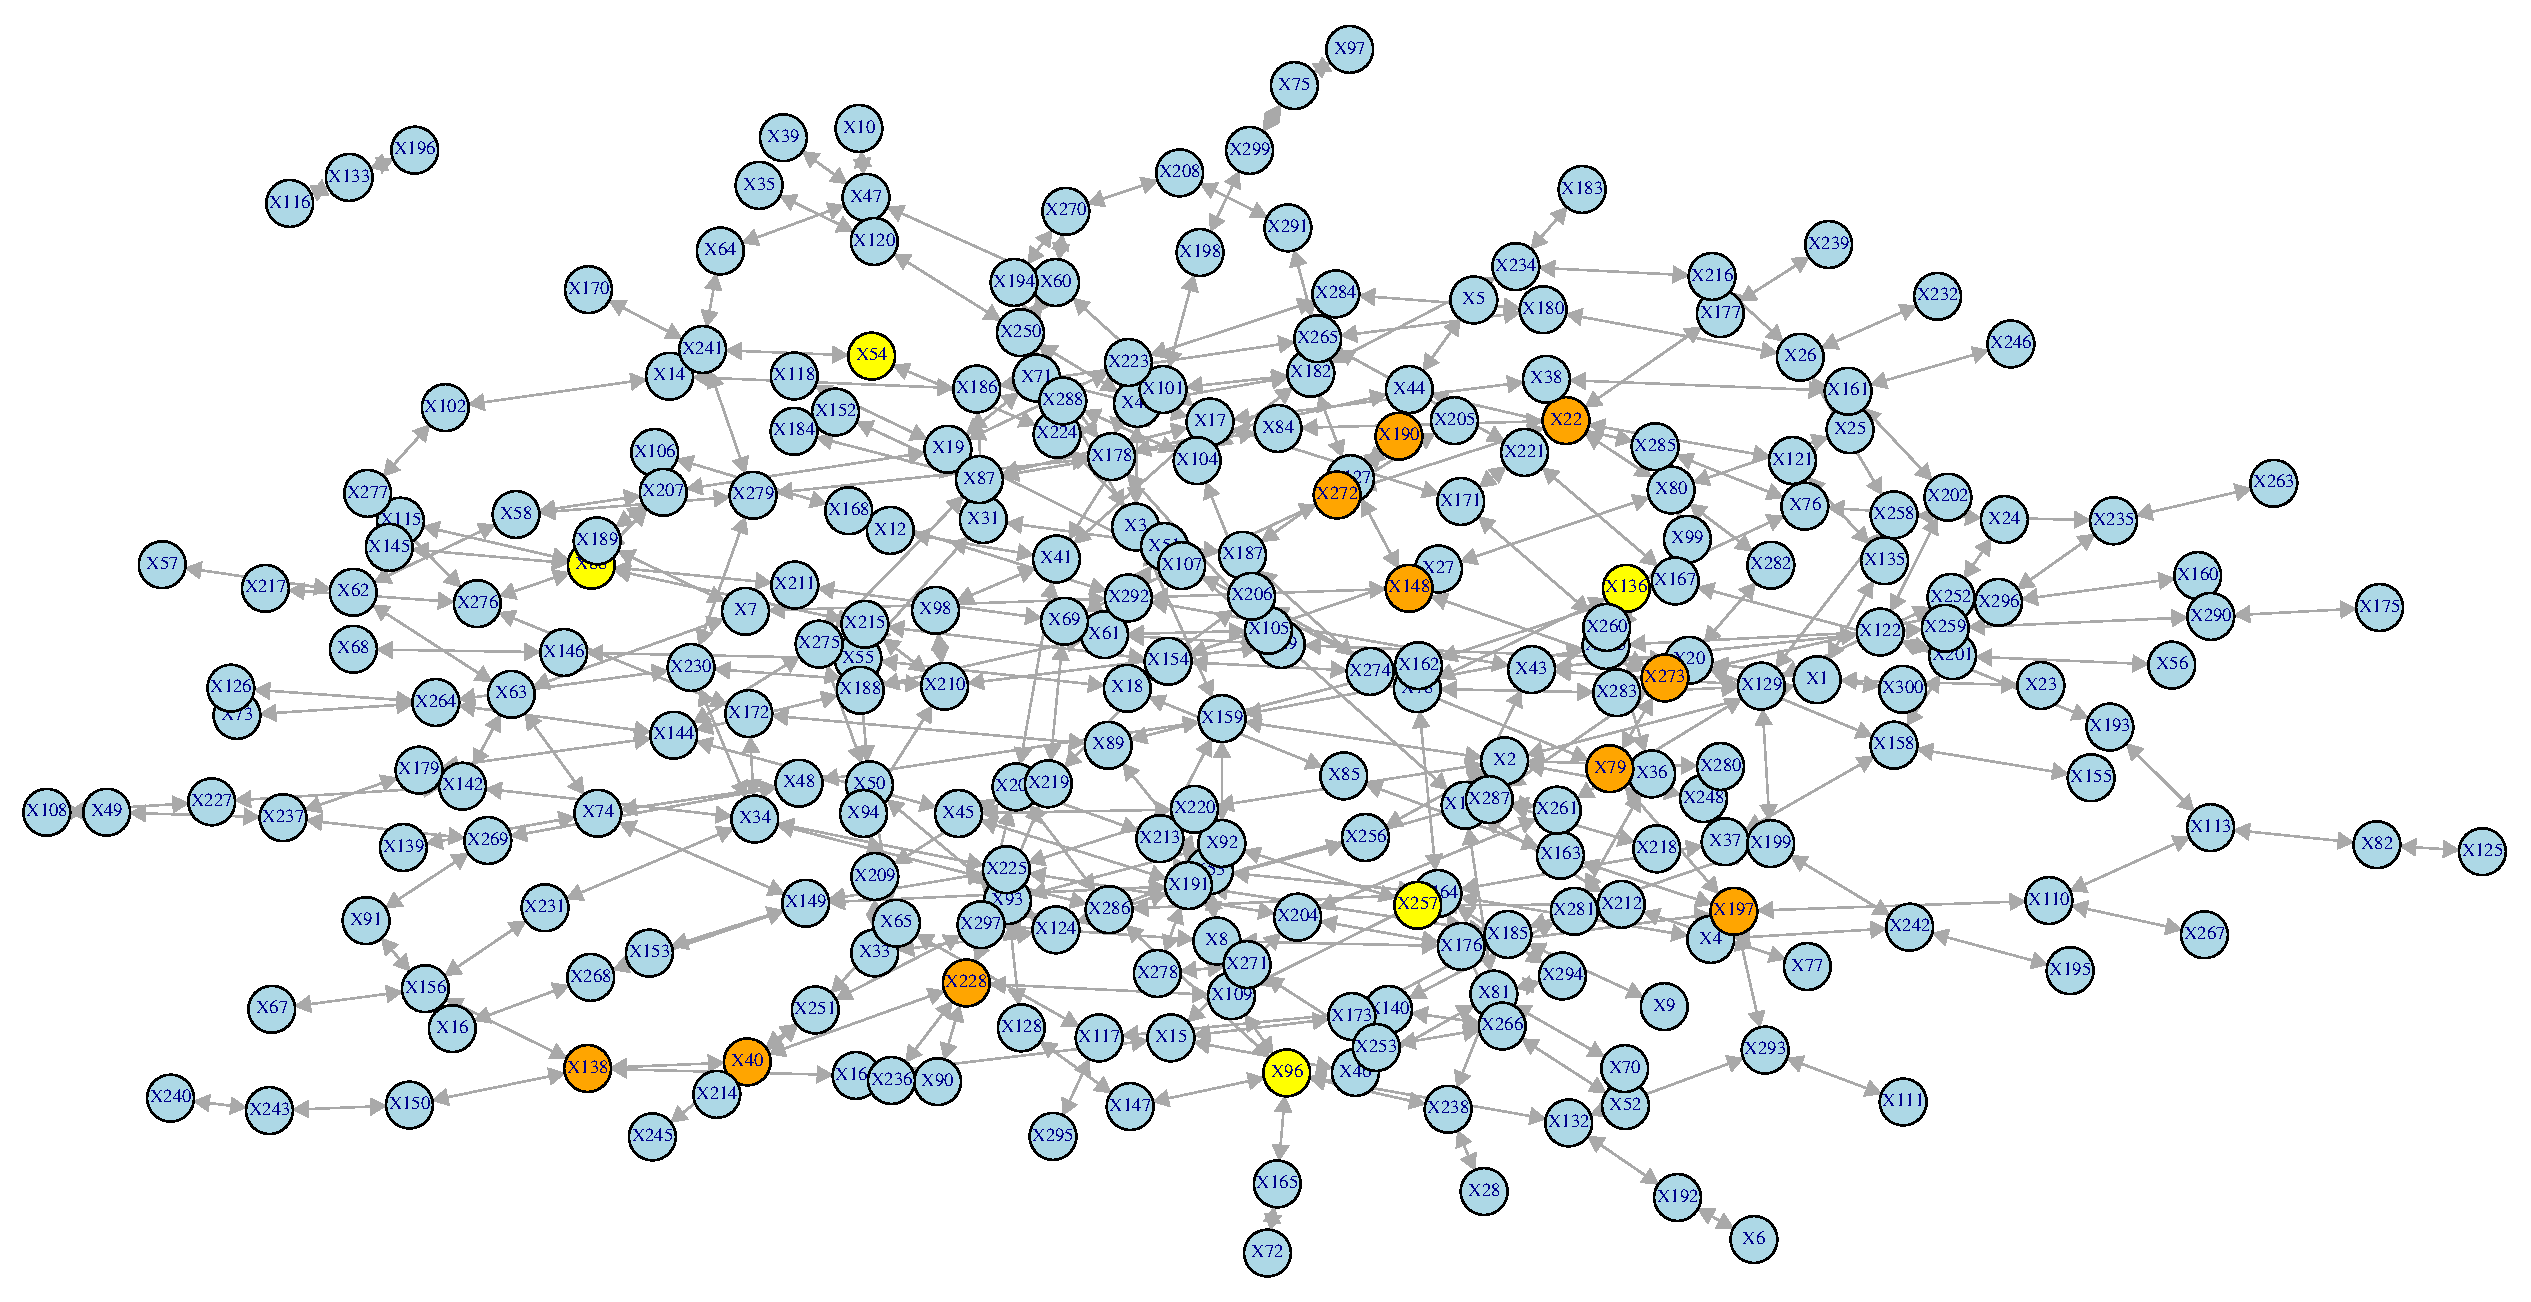
\includegraphics[width=0.8\textwidth]{synthesized-hard}
  \end{figure}
  \begin{textblock*}{\paperwidth}(0.01\textwidth,0.15\textheight)
    \raggedright 
    \tiny
    \begin{tabular}{| c c |}
      \hline
AUC: & 60.2 \\ \hline \hline
\boz X190   &  \boz X190  \\ \hline
X101   &  X101  \\ \hline
X233   &  X233  \\ \hline
\boz X190   &  \boz X272  \\ \hline
\ghool X88   &  \ghool X88  \\ \hline
X297   &  X297  \\ \hline
\boz X190   &  X127  \\ \hline
X93   &  X93  \\ \hline
X26   &  X26  \\ \hline
\boz X138   &  \boz X138  \\ \hline
\boz X272   &  \boz X272  \\ \hline
\boz X272   &  \boz X22  \\ \hline
X101   &  X41  \\ \hline
X123   &  X123  \\ \hline
\boz X22   &  \boz X22  \\ \hline
X101   &  X198  \\ \hline
X146   &  X146  \\ \hline
\boz X228   &  \boz X228  \\ \hline
X278   &  X278  \\ \hline
X72   &  X72  \\ \hline
\ghool X88   &  X115  \\ \hline
\ghool X96   &  \ghool X96  \\ \hline
\boz X148   &  \boz X148  \\ \hline
X112   &  X112  \\ \hline
X35   &  X35  \\ \hline
\ghool X96   &  X132  \\ \hline
X161   &  X161  \\ \hline
X155   &  X155  \\ \hline
X297   &  X251  \\ \hline
\boz X138   &  X169  \\ \hline
    \end{tabular}
    \hspace{.5em}
  \end{textblock*}
  \begin{textblock*}{\paperwidth}(1\textwidth,0.15\textheight)
    \raggedright 
    \tiny
    \begin{tabular}{| c c |}
      \hline
AUC: & 62.5 \\ \hline \hline
X233   &  X233  \\ \hline
\boz X190   &  \boz X190  \\ \hline
X112   &  X112  \\ \hline
\boz X190   &  \boz X272  \\ \hline
X86   &  X86  \\ \hline
\boz X190   &  X127  \\ \hline
\boz X272   &  \boz X272  \\ \hline
\boz X272   &  X205  \\ \hline
X205   &  X205  \\ \hline
X146   &  X146  \\ \hline
X146   &  X68  \\ \hline
X68   &  X68  \\ \hline
X298   &  X298  \\ \hline
\boz X272   &  \boz X22  \\ \hline
X90   &  X90  \\ \hline
X127   &  X127  \\ \hline
X100   &  X100  \\ \hline
\boz X272   &  X69  \\ \hline
X297   &  X297  \\ \hline
X72   &  X72  \\ \hline
X127   &  \boz X148  \\ \hline
X155   &  X155  \\ \hline
X247   &  X247  \\ \hline
X196   &  X196  \\ \hline
\boz X148   &  \boz X148  \\ \hline
X101   &  X101  \\ \hline
X21   &  X21  \\ \hline
X106   &  X106  \\ \hline
X90   &  \boz X228  \\ \hline
X297   &  X251  \\ \hline
    \end{tabular}
    \hspace{.5em}
  \end{textblock*}
  \begin{textblock*}{\paperwidth}(0.4\textwidth,1.1\textheight)
    \raggedright 
    \tiny
    \begin{tabular}{| c c |}
      \hline
      wc p-value (paired): & 8.151e-13 \\ \hline
    \end{tabular}
    \hspace{.5em}
  \end{textblock*}
\end{frame}

\begin{frame}[plain]
  \frametitle{Van't Veer}
  \begin{textblock*}{\paperwidth}(0.01\textwidth,0.25\textheight)
    \raggedright 
    \tiny
    \begin{tabular}{| c c |}
      \hline
AUC: & 72.9 \\ \hline \hline
X85453  &  X85453 \\ \hline 
X85453  &  X92140 \\ \hline 
X6605  &  X6605 \\ \hline 
X56886  &  X56886 \\ \hline 
X10640  &  X10640 \\ \hline 
X8817  &  X8817 \\ \hline 
X56894  &  X56894 \\ \hline 
X6605  &  X332 \\ \hline 
X5733  &  X5733 \\ \hline 
X57758  &  X57758 \\ \hline 
X7532  &  X7532 \\ \hline 
X51  &  X51 \\ \hline 
X7566  &  X7566 \\ \hline 
X3267  &  X3267 \\ \hline 
X89953  &  X89953 \\ \hline 
X5713  &  X5713 \\ \hline 
X5193  &  X5193 \\ \hline 
X5365  &  X5365 \\ \hline 
X10874  &  X10874 \\ \hline 
X5982  &  X5982 \\ \hline 
    \end{tabular}
    \hspace{.5em}
  \end{textblock*}
  \begin{textblock*}{\paperwidth}(0.93\textwidth,0.25\textheight)
    \raggedright 
    \tiny
    \begin{tabular}{| c c |}
      \hline
AUC: & 73.6 \\ \hline \hline
X9917  &  X9917 \\ \hline 
X84279  &  X84279 \\ \hline 
X197370  &  X197370 \\ \hline 
X51143  &  X51143 \\ \hline 
X58475  &  X58475 \\ \hline 
X55585  &  X55585 \\ \hline 
X25949  &  X25949 \\ \hline 
X54892  &  X54892 \\ \hline 
X126695  &  X126695 \\ \hline 
X57168  &  X57168 \\ \hline 
X10456  &  X10456 \\ \hline 
X148223  &  X148223 \\ \hline 
X9742  &  X9742 \\ \hline 
X253558  &  X253558 \\ \hline 
X342527  &  X342527 \\ \hline 
X10175  &  X10175 \\ \hline 
X83930  &  X83930 \\ \hline 
X57035  &  X57035 \\ \hline 
X145482  &  X145482 \\ \hline 
X57465  &  X57465 \\ \hline 
    \end{tabular}
    \hspace{.5em}
  \end{textblock*}
  \begin{textblock*}{\paperwidth}(0.4\textwidth,1.1\textheight)
    \raggedright 
    \tiny
    \begin{tabular}{| c c |}
      \hline
      wc p-value (paired): & 0.006 \\ \hline
    \end{tabular}
    \hspace{.5em}
  \end{textblock*}
\only<2>{
  \begin{textblock*}{\paperwidth}(0.26\textwidth,0.3\textheight)
    \raggedright 
    \tiny
    \begin{tabular}{| c c |}
      \hline
\cellcolor[gray]{0.8} Node & \cellcolor[gray]{0.8} Degree \\ \hline
X85453  &  12 \\ \hline 
X6605  &  98 \\ \hline 
X56886  &  26 \\ \hline 
X10640  &  16 \\ \hline 
X8817  &  152 \\ \hline 
X56894  &  28 \\ \hline 
X5733  &  150 \\ \hline 
X57758  &  8 \\ \hline 
X7532  &  86 \\ \hline 
X51  &  172 \\ \hline 
X7566  &  16 \\ \hline 
X3267  &  56 \\ \hline 
X89953  &  4 \\ \hline 
X5713  &  126 \\ \hline 
X5193  &  32 \\ \hline 
X5365  &  70 \\ \hline 
X10874  &  132 \\ \hline 
X5982  &  172 \\ \hline 
X92140  &  20 \\ \hline 
X332  &  328 \\ \hline 
    \end{tabular}
    \hspace{.5em}
  \end{textblock*}
  \begin{textblock*}{\paperwidth}(0.68\textwidth,0.3\textheight)
    \raggedright 
    \tiny
    \begin{tabular}{| c c |}
      \hline
\cellcolor[gray]{0.8} Node & \cellcolor[gray]{0.8} Degree \\ \hline
X9917  &  0 \\ \hline 
X84279  &  0 \\ \hline 
X197370  &  0 \\ \hline 
X51143  &  0 \\ \hline 
X58475  &  0 \\ \hline 
X55585  &  0 \\ \hline 
X25949  &  0 \\ \hline 
X54892  &  0 \\ \hline 
X126695  &  0 \\ \hline 
X57168  &  0 \\ \hline 
X10456  &  0 \\ \hline 
X148223  &  0 \\ \hline 
X9742  &  0 \\ \hline 
X253558  &  0 \\ \hline 
X342527  &  0 \\ \hline 
X10175  &  0 \\ \hline 
X83930  &  0 \\ \hline 
X57035  &  0 \\ \hline 
X145482  &  0 \\ \hline 
X57465  &  0 \\ \hline 
    \end{tabular}
    \hspace{.5em}
  \end{textblock*}
}
\end{frame}

\section{Work in progress}
\begin{frame}
  \frametitle{Idea}
  \begin{enumerate}
\footnotesize
  \item Estimate gene expression value probability distributions for samples of class A. \pause
  \item For each sample in class A and B:
    \begin{enumerate}
    \item Extract abnormal genes according to above estimated distributions.
    \item Extract the part of PPI network induced by extracted genes (almost)
    \end{enumerate}\pause
  \item Use a graph kernel for labeled graphs to classify extracted graphs. \pause
  \item Extract common sub-graphs from individual graphs that seem to be helping the classification. \pause
  \end{enumerate}
\only<5>{
  \begin{textblock*}{\paperwidth}(0.4\textwidth,0.85\textheight)
    \raggedright
  \begin{figure}
    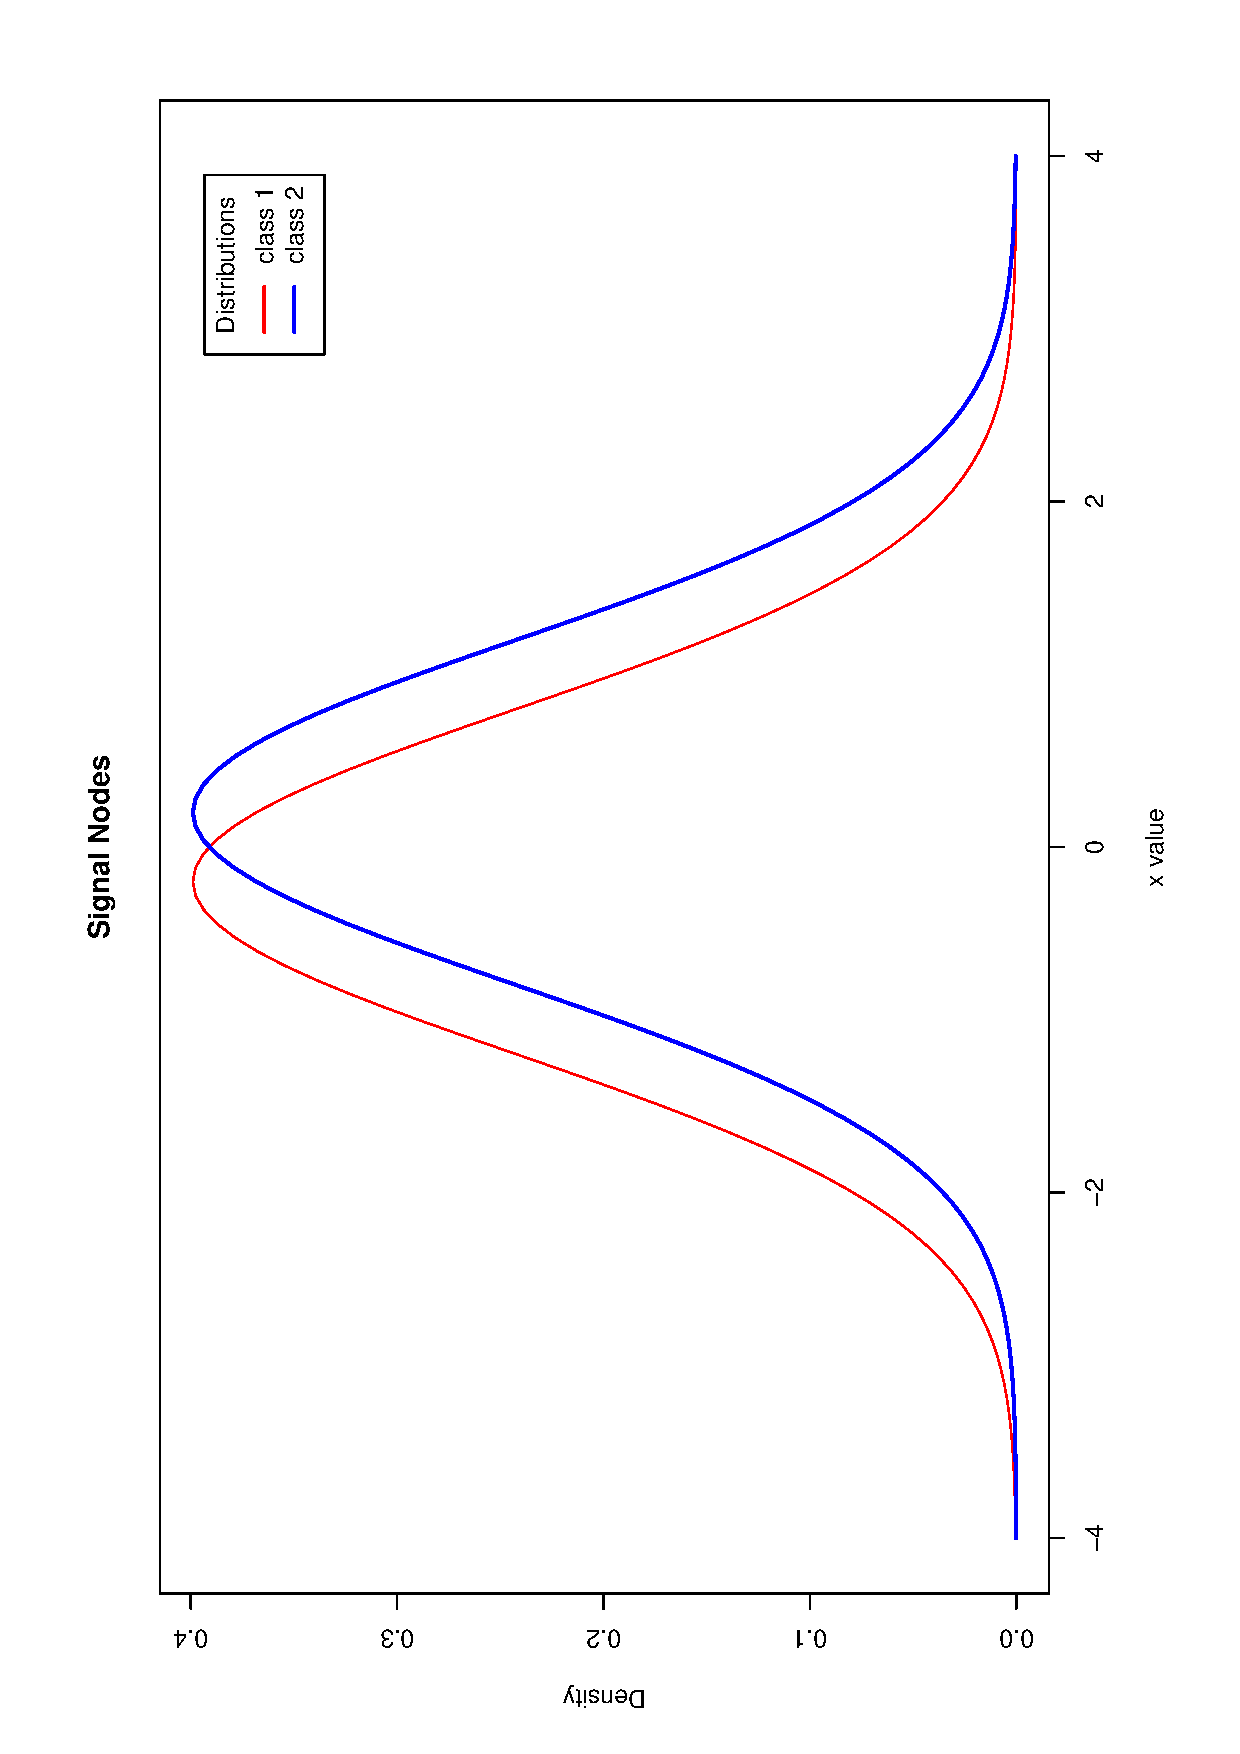
\includegraphics[angle=270,width=0.2\textwidth]{signal-nodes}
  \end{figure}
  \end{textblock*}
}
\end{frame}

\begin{frame}[plain]
  \frametitle{Weighted idea}
\only<1>{
  \begin{figure}
    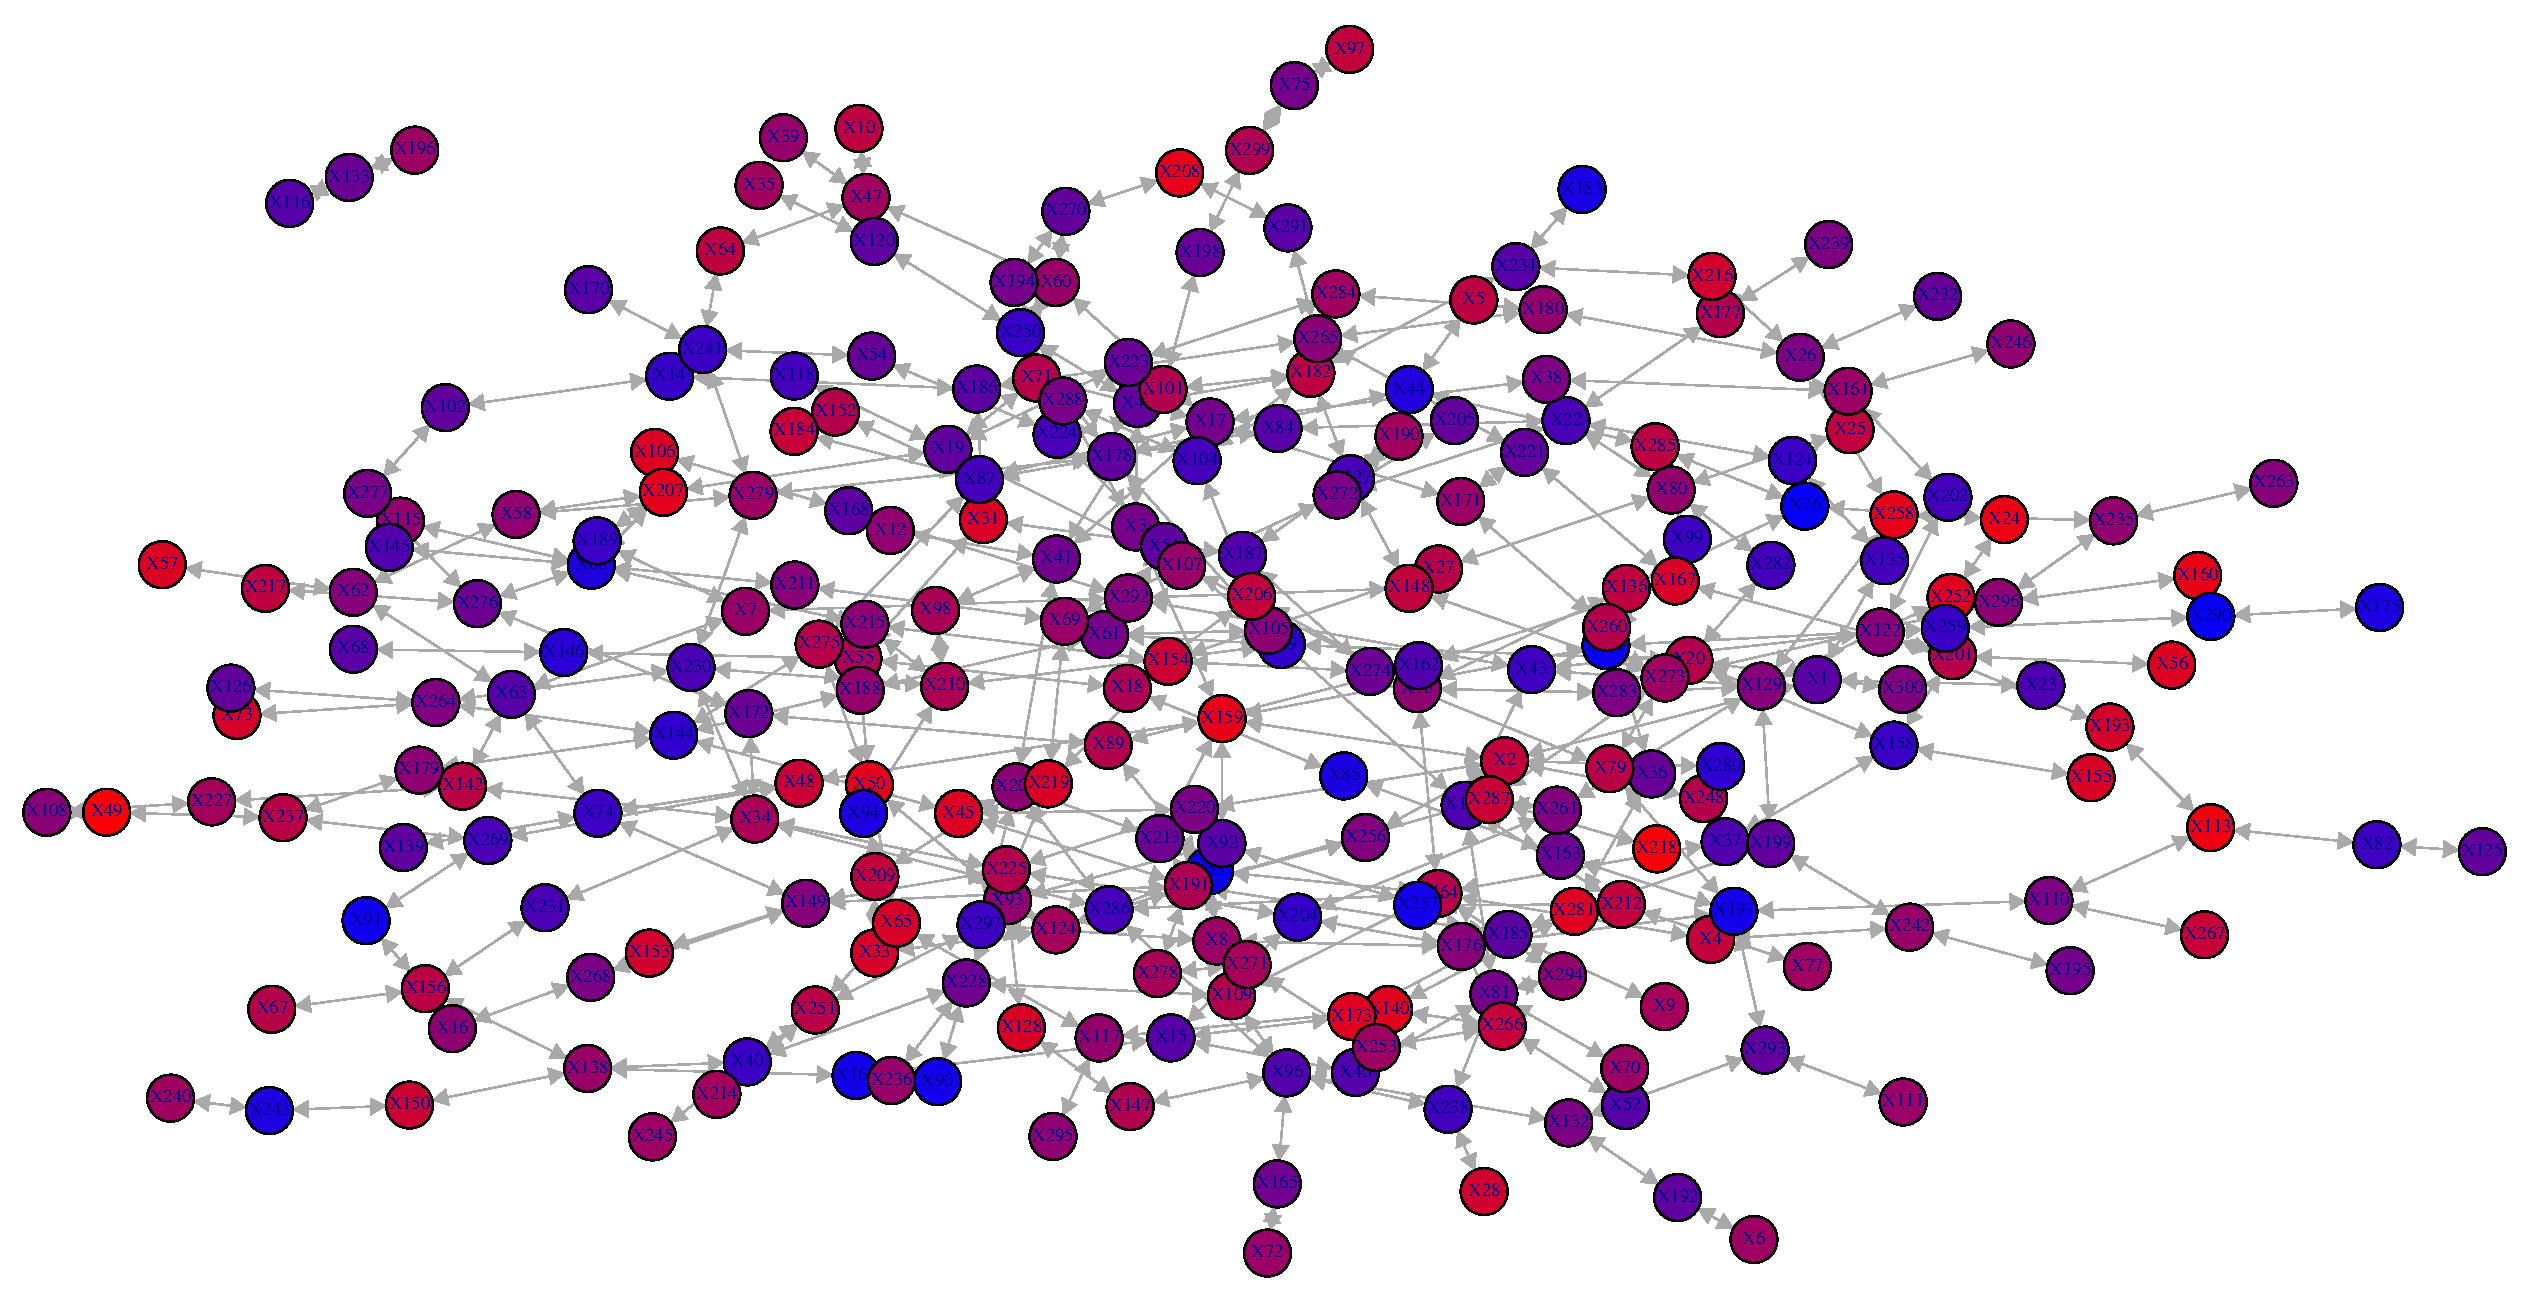
\includegraphics[width=1\textwidth]{weighted-1}
    \caption{Class A member}
  \end{figure}
}
\only<2>{
  \begin{figure}
    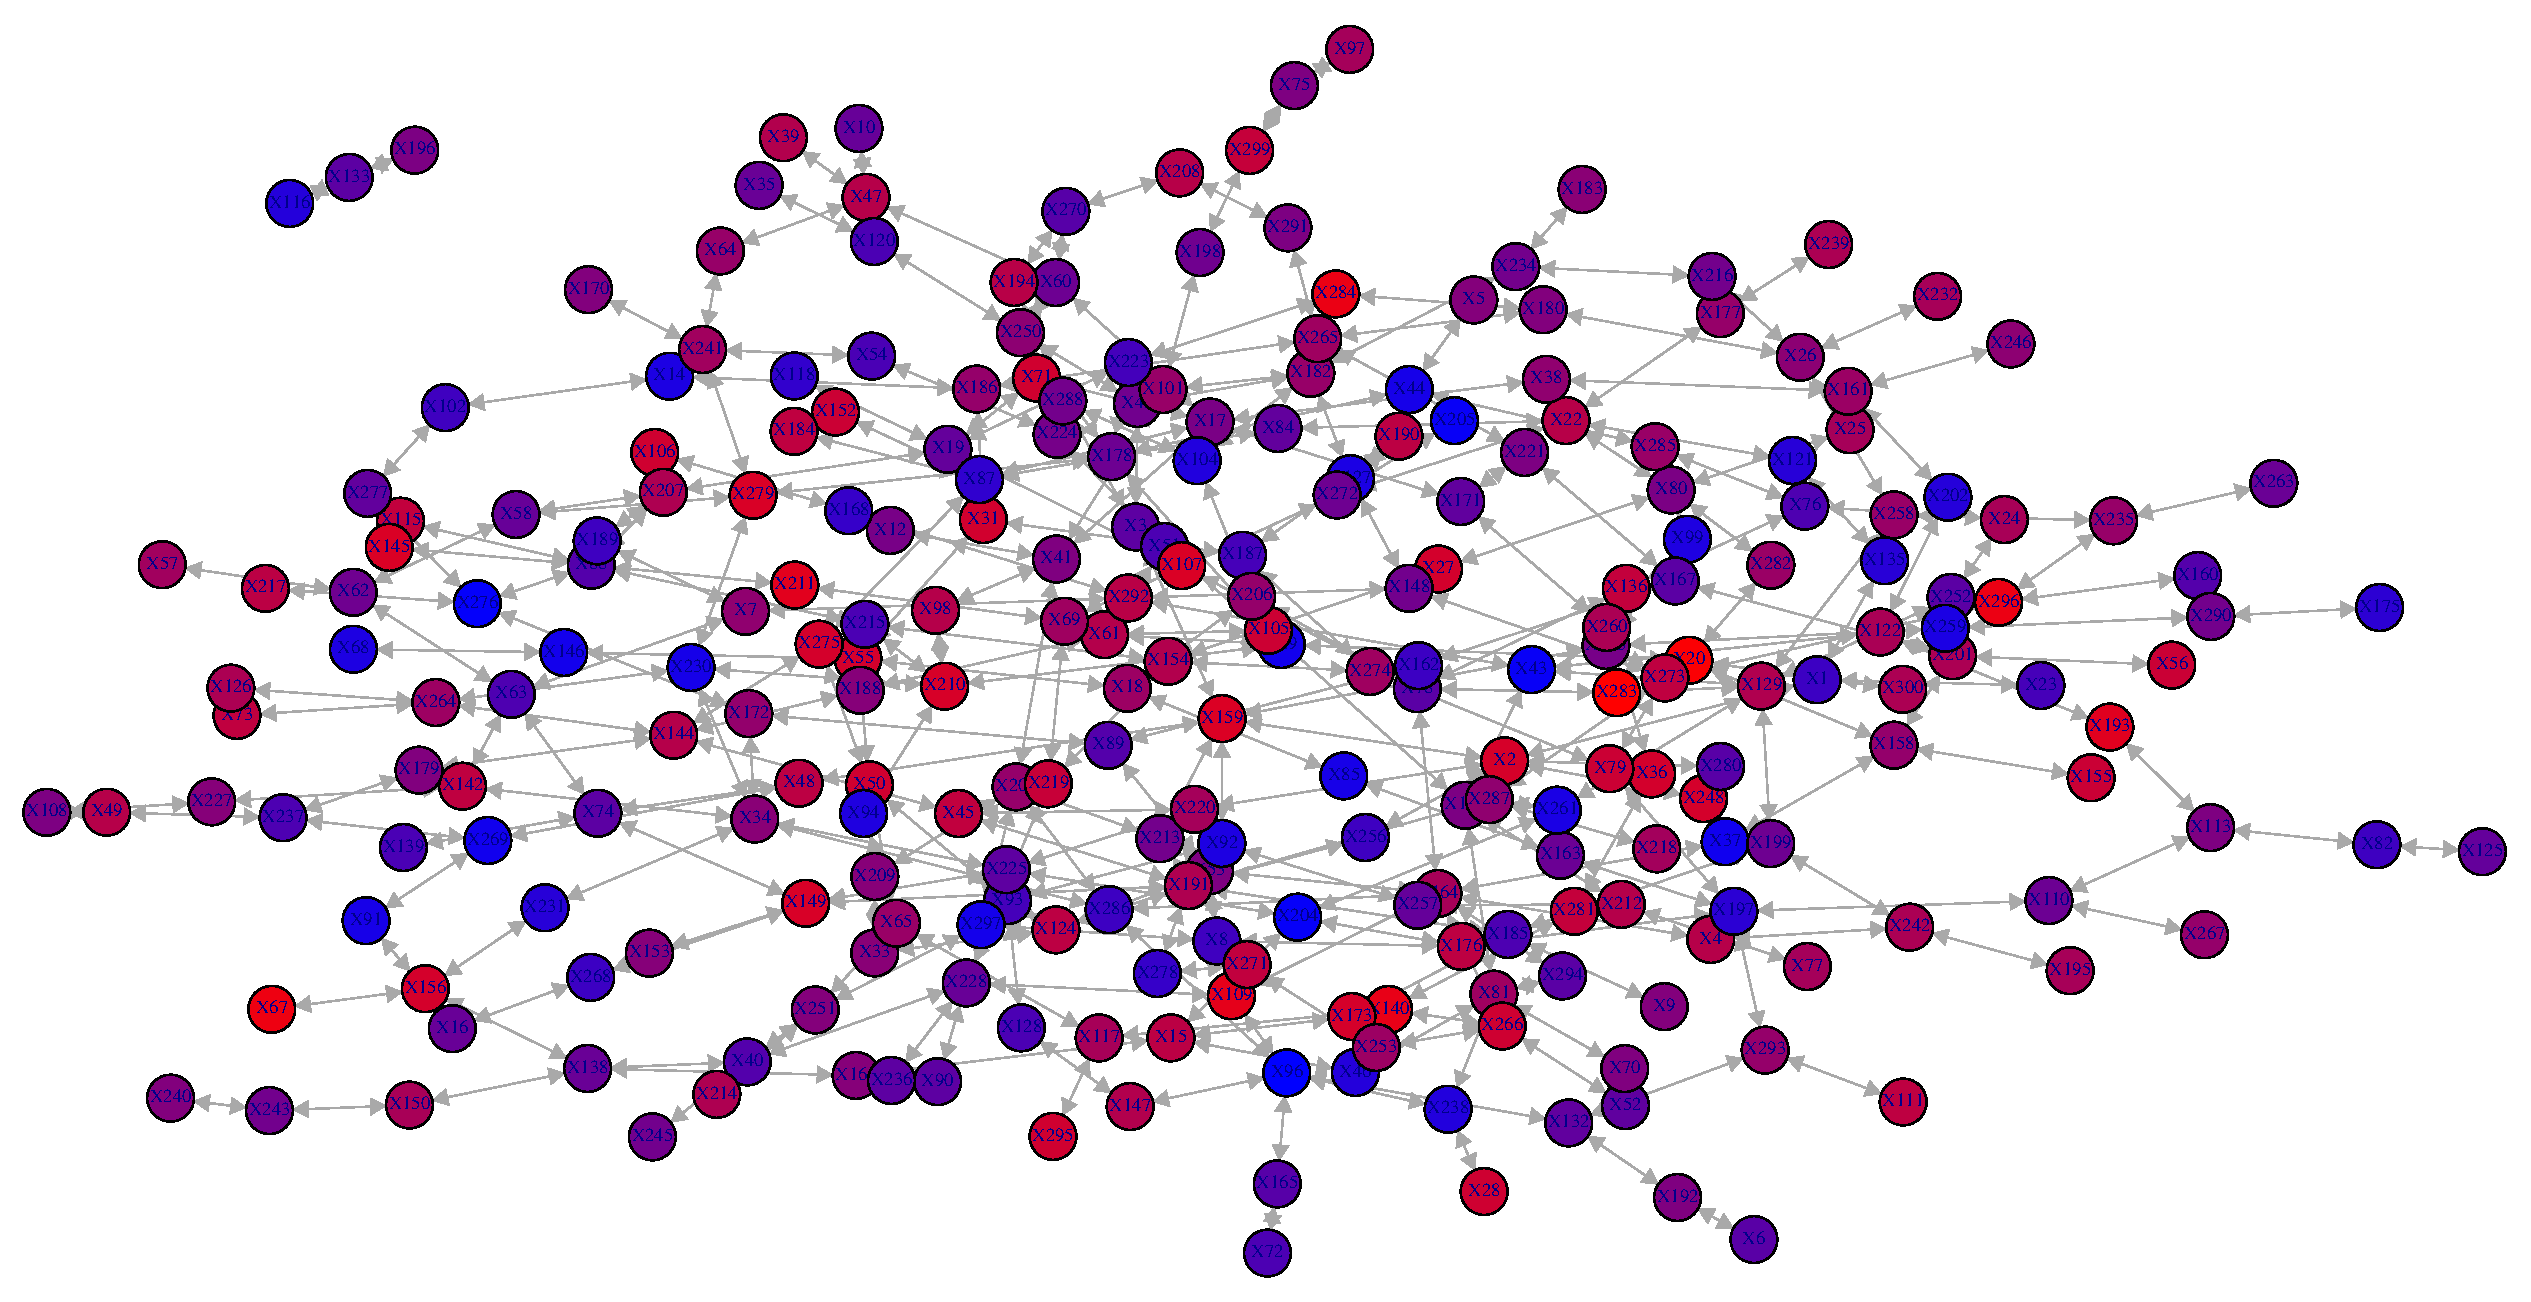
\includegraphics[width=1\textwidth]{weighted-2}
    \caption{Class B member}
  \end{figure}
}
\end{frame}

\begin{frame}[plain]
\frametitle{Finished!}
  \begin{center}
    \Huge{Thank You!}\\
    Questions?
  \end{center}
\end{frame}

\end{document}
